\documentclass[12pt,a4paper]{report}

\usepackage[utf8]{inputenc}
\usepackage[T1]{fontenc}
\usepackage[margin=1in]{geometry}
\usepackage{amsmath,amssymb,amsthm}
\usepackage{mathtools}
\usepackage{hyperref}
\usepackage{cleveref}
\usepackage{booktabs}
\usepackage{enumitem}
\usepackage{xcolor}
\usepackage{fancyhdr}
\usepackage{setspace}
\usepackage{natbib}
\usepackage{tikz}
\usetikzlibrary{positioning}
\usepackage{algorithm}
\usepackage{algpseudocode}

\onehalfspacing
\pagestyle{fancy}
\fancyhf{}
\fancyhead[R]{\textit{\small Boolean Fourier Analysis: An Expository Guide}}
\fancyfoot[C]{\thepage}
\renewcommand{\headrulewidth}{0.4pt}

% ── Theorem environments ──────────────────────────────────────────────
\theoremstyle{plain}
\newtheorem{theorem}{Theorem}[section]
\newtheorem{lemma}[theorem]{Lemma}
\newtheorem{proposition}[theorem]{Proposition}
\newtheorem{corollary}[theorem]{Corollary}

\theoremstyle{definition}
\newtheorem{definition}[theorem]{Definition}
\newtheorem{example}[theorem]{Example}

\theoremstyle{remark}
\newtheorem{remark}[theorem]{Remark}

% ── Macros ────────────────────────────────────────────────────────────
\newcommand{\R}{\mathbb{R}}
\newcommand{\Z}{\mathbb{Z}}
\newcommand{\N}{\mathbb{N}}
\newcommand{\E}{\mathbb{E}}
\newcommand{\Prob}{\mathbb{P}}
\newcommand{\pmone}{\{-1,+1\}}
\newcommand{\fhat}{\widehat{f}}
\newcommand{\ghat}{\widehat{g}}
\newcommand{\ip}[2]{\langle #1, #2 \rangle}
\newcommand{\norm}[1]{\left\| #1 \right\|}
\newcommand{\abs}[1]{\left| #1 \right|}
\newcommand{\Var}{\operatorname{Var}}
\newcommand{\Inf}{\operatorname{Inf}}
\newcommand{\Stab}{\operatorname{Stab}}
\newcommand{\sgn}{\operatorname{sgn}}
\DeclareMathOperator{\WHT}{WHT}
\DeclareMathOperator{\FWHT}{FWHT}

\begin{document}

% ── Title page ────────────────────────────────────────────────────────
\begin{titlepage}
\centering
\vspace*{2cm}

{\LARGE\bfseries Boolean Fourier Analysis and the\\[6pt]
Walsh--Hadamard Transform}\\[18pt]
{\Large\bfseries An Expository Guide}\\[12pt]
{\large From First Principles to Spectral Methods\\[4pt]
for Binary Neural Networks}

\vspace{2cm}

{\large Companion to the thesis proposal:\\[4pt]
\textit{Spectral Methods for Binary Neural Networks}}

\vspace{1.5cm}

{\large February 2026}

\vspace{2cm}

\begin{quote}\small
This document provides a self-contained exposition of the mathematical
background needed to read the thesis proposal on spectral methods for
binary neural networks. It assumes familiarity with undergraduate linear
algebra, probability, and calculus, but develops all specialized material---Boolean
Fourier analysis, the Walsh--Hadamard transform, hypercontractivity,
influence theory, and their connections to coding theory and neural
networks---from scratch, with full proofs and references.
\end{quote}

\end{titlepage}

\tableofcontents
\newpage

% ══════════════════════════════════════════════════════════════════════════
%  Chapter 1: Prerequisites
% ══════════════════════════════════════════════════════════════════════════

\chapter{Prerequisites}\label{ch:prereqs}

We collect the facts from linear algebra and probability that are used
throughout this guide. The reader who is comfortable with inner product
spaces, the Kronecker product, Markov's inequality, and the central limit
theorem may safely skip to \Cref{ch:boolean-fourier}.

Standard references: \citet{axler2024linear} or \citet{horn2012matrix} for
linear algebra; \citet{durrett2019probability} or \citet{feller1971introduction}
for probability.

% ──────────────────────────────────────────────────────────────────────
\section{Inner Product Spaces}\label{sec:inner-product-spaces}

\begin{definition}[Inner product]\label{def:inner-product}
Let $V$ be a real vector space. An \emph{inner product}\index{inner product} on $V$ is a
function $\ip{\cdot}{\cdot} \colon V \times V \to \R$ satisfying, for all
$u, v, w \in V$ and $\alpha \in \R$:
\begin{enumerate}[label=(\roman*)]
  \item \emph{Symmetry:} $\ip{u}{v} = \ip{v}{u}$.
  \item \emph{Linearity in the first argument:}
        $\ip{\alpha u + v}{w} = \alpha\ip{u}{w} + \ip{v}{w}$.
  \item \emph{Positive definiteness:} $\ip{v}{v} \geq 0$, with equality
        if and only if $v = 0$.
\end{enumerate}
The pair $(V, \ip{\cdot}{\cdot})$ is called an \emph{inner product space}.
\end{definition}

The inner product induces a norm $\norm{v} = \sqrt{\ip{v}{v}}$.
The key structural fact is:

\begin{theorem}[Cauchy--Schwarz inequality]\label{thm:cauchy-schwarz}
For all $u, v$ in an inner product space,
$|\ip{u}{v}| \leq \norm{u}\,\norm{v}$,
with equality if and only if $u$ and $v$ are linearly dependent.%
\footnote{Proof: see \citet[Chapter~6]{axler2024linear} or
\citet[Section~5.1]{horn2012matrix}.}
\end{theorem}

\begin{definition}[Orthonormal basis]\label{def:onb}
A set $\{e_1, \ldots, e_n\}$ in an inner product space $V$ is
\emph{orthonormal} if $\ip{e_i}{e_j} = \delta_{ij}$ (the Kronecker delta).
If additionally $\operatorname{span}\{e_1,\ldots,e_n\} = V$, it is an
\emph{orthonormal basis} (ONB).
\end{definition}

The central fact about orthonormal bases is:

\begin{proposition}[Fourier expansion in a finite-dimensional inner product space]\label{prop:fourier-finite}
If $\{e_1, \ldots, e_N\}$ is an ONB for $(V, \ip{\cdot}{\cdot})$, then
every $v \in V$ has a unique expansion
\[
  v = \sum_{i=1}^{N} \ip{v}{e_i}\, e_i,
\]
and \emph{Parseval's identity} holds:
$\norm{v}^2 = \sum_{i=1}^{N} \ip{v}{e_i}^2$.
\end{proposition}

\begin{proof}
Write $v = \sum_i c_i e_i$. Taking the inner product with $e_j$ gives
$\ip{v}{e_j} = c_j$ by orthonormality. Then
$\norm{v}^2 = \ip{v}{v} = \sum_i c_i^2$.
\end{proof}

This is exactly the abstract template for the Boolean Fourier expansion
in \Cref{ch:boolean-fourier}: the vector space will be the space of all
real-valued functions on $\pmone^n$, the inner product will be the
expectation inner product, and the ONB will be the parity functions.


% ──────────────────────────────────────────────────────────────────────
\section{The Kronecker Product}\label{sec:kronecker}

\begin{definition}[Kronecker product]\label{def:kronecker}
Let $A$ be an $m \times n$ matrix and $B$ a $p \times q$ matrix. Their
\emph{Kronecker product}\index{Kronecker product} $A \otimes B$ is the $mp \times nq$ block matrix
\[
  A \otimes B =
  \begin{pmatrix}
    a_{11} B & a_{12} B & \cdots & a_{1n} B \\
    a_{21} B & a_{22} B & \cdots & a_{2n} B \\
    \vdots & \vdots & \ddots & \vdots \\
    a_{m1} B & a_{m2} B & \cdots & a_{mn} B
  \end{pmatrix}.
\]
\end{definition}

Key properties (all straightforward to verify; see
\citealp[Chapter~4]{horn2012matrix} for proofs):
\begin{enumerate}[label=(\roman*)]
  \item $(A \otimes B)(C \otimes D) = (AC) \otimes (BD)$, when the
        products $AC$ and $BD$ are defined.
  \item $(A \otimes B)^\top = A^\top \otimes B^\top$.
  \item If $A$ and $B$ are orthogonal ($A^\top A = I$ and $B^\top B = I$),
        so is $A \otimes B$. (More generally, if $A^\top A = \alpha I$
        and $B^\top B = \beta I$, then
        $(A \otimes B)^\top(A \otimes B) = \alpha\beta \cdot I$.)
  \item $\operatorname{tr}(A \otimes B) = \operatorname{tr}(A)\operatorname{tr}(B)$.
\end{enumerate}

Property (i) is the \emph{mixed-product rule}; it is the algebraic engine
behind the recursive structure of the Hadamard matrix (\Cref{ch:wht}).

\begin{example}[Mixed-product rule]\label{ex:mixed-product}
Let $A = \bigl(\begin{smallmatrix} 1 & 1 \\ 1 & -1 \end{smallmatrix}\bigr) = H_1$.
Then $(H_1 \otimes H_1)(H_1 \otimes H_1) = (H_1 H_1) \otimes (H_1 H_1)
= (2I_2) \otimes (2I_2) = 4I_4$. This verifies that $H_2^2 = 4I_4$
(which we will prove in general in \Cref{ch:wht}).
\end{example}

\begin{example}\label{ex:kronecker-2x2}
The Hadamard matrix $H_1 = \bigl(\begin{smallmatrix} 1 & 1 \\ 1 & -1
\end{smallmatrix}\bigr)$ satisfies
\[
  H_1 \otimes H_1 =
  \begin{pmatrix}
    1 & 1 & 1 & 1 \\
    1 & -1 & 1 & -1 \\
    1 & 1 & -1 & -1 \\
    1 & -1 & -1 & 1
  \end{pmatrix} = H_2.
\]
See \Cref{sec:hadamard-def} for the general construction.
\end{example}


% ──────────────────────────────────────────────────────────────────────
\section{Probability Essentials}\label{sec:prob-essentials}

Throughout this guide, probability spaces are finite (typically uniform
on $\pmone^n$), so measure-theoretic subtleties do not arise.

\begin{definition}[Expectation and variance]\label{def:expectation}
For a random variable $X$ on a finite probability space
$(\Omega, \mu)$ (where $\mu(\omega)$ is the probability of outcome $\omega$):
\[
  \E[X] = \sum_{\omega \in \Omega} \mu(\omega)\, X(\omega),
  \qquad
  \Var[X] = \E[(X - \E[X])^2] = \E[X^2] - (\E[X])^2.
\]
\end{definition}

\begin{theorem}[Markov's inequality]\label{thm:markov}\index{Markov's inequality}
If $X \geq 0$ and $a > 0$, then $\Prob[X \geq a] \leq \E[X] / a$.
\end{theorem}

\begin{proof}
$\E[X] = \sum_\omega \mu(\omega) X(\omega) \geq \sum_{\omega : X(\omega) \geq a} \mu(\omega) \cdot a = a \cdot \Prob[X \geq a]$.
\end{proof}

\begin{corollary}[Chebyshev's inequality]\label{cor:chebyshev}\index{Chebyshev's inequality}
$\Prob[|X - \E[X]| \geq t] \leq \Var[X] / t^2$.
\end{corollary}

\begin{proof}
Apply Markov to $(X - \E[X])^2$ with $a = t^2$.
\end{proof}

Markov's inequality is used directly in the thesis to prove the
degree-truncation approximation bound (Proposition~3.1 of the thesis).


% ──────────────────────────────────────────────────────────────────────
\section{The Central Limit Theorem and Berry--Ess\'een}\label{sec:clt}

\begin{theorem}[Central Limit Theorem]\label{thm:clt}\index{central limit theorem}
Let $X_1, X_2, \ldots$ be independent, identically distributed random
variables with $\E[X_i] = 0$ and $\Var[X_i] = \sigma^2 > 0$. Write
$S_n = X_1 + \cdots + X_n$ for the partial sum. Then
\[
  \frac{S_n}{\sigma\sqrt{n}}
  \xrightarrow{d} \mathcal{N}(0, 1)
  \quad \text{as } n \to \infty.
\]
Here $\xrightarrow{d}$ denotes \emph{convergence in distribution}:
$\Prob[S_n / (\sigma\sqrt{n}) \leq t] \to \Phi(t)$ for every $t$,
where $\Phi(t) = \frac{1}{\sqrt{2\pi}}\int_{-\infty}^t e^{-s^2/2}\,ds$
is the standard normal CDF.%
\footnote{For proof via characteristic functions, see
\citet[Chapter~3]{durrett2019probability} or
\citet[Chapter~XV]{feller1971introduction}.}
\end{theorem}

The CLT tells us that $S_n / (\sigma \sqrt{n})$ is approximately
$\mathcal{N}(0,1)$ for large $n$, but says nothing about the rate of
convergence. The Berry--Ess\'een theorem quantifies this.

\begin{theorem}[Berry--Ess\'een; \citealp{berry1941accuracy,esseen1942rate}]\label{thm:berry-esseen}\index{Berry--Ess\'een theorem}
Under the hypotheses of \Cref{thm:clt}, with additionally
$\E[|X_i|^3] = \gamma < \infty$, we have
\[
  \sup_{t \in \R}
  \left|
    \Prob\!\left[\frac{S_n}{\sigma\sqrt{n}} \leq t\right]
    - \Phi(t)
  \right|
  \leq \frac{C \gamma}{\sigma^3 \sqrt{n}},
\]
where $C$ is a universal constant (the best known value is $C < 0.4748$;
see \citealp{shevtsova2011absolute}).
\end{theorem}

\paragraph{Why this matters for the thesis.}
In the thesis, binary neural network layers compute sums of the form
$y_j = \sum_{i=1}^d w_{ji} x_i$ where $w_{ji}, x_i \in \pmone$.
When $x$ is uniform on $\pmone^d$, the summands $w_{ji} x_i$ are
independent $\pm 1$ random variables (regardless of the fixed signs
$w_{ji}$), so $\E[w_{ji} x_i] = 0$, $\Var[w_{ji} x_i] = 1$, and
$\E[|w_{ji} x_i|^3] = 1$. By Berry--Ess\'een,
$y_j / \sqrt{d}$ is within $O(1/\sqrt{d})$ of $\mathcal{N}(0,1)$ in CDF.
At $d = 1024$, this is about $0.015$---excellent approximation.
This justifies the $1/\sqrt{d}$ normalization used throughout the thesis
as a replacement for BitNet's learned scaling factors.


% ──────────────────────────────────────────────────────────────────────
\section{$L^p$ Norms}\label{sec:lp-norms}

For a function $f$ on a probability space $(\Omega, \mu)$:

\begin{definition}[$L^p$ norm]\label{def:lp}
For $p \geq 1$:
\[
  \norm{f}_p = \left(\E\!\left[|f|^p\right]\right)^{1/p}
  = \left(\sum_{\omega \in \Omega} \mu(\omega)\, |f(\omega)|^p\right)^{1/p}.
\]
For $p = \infty$: $\norm{f}_\infty = \max_\omega |f(\omega)|$.
\end{definition}

On a probability space, we always have $\norm{f}_p \leq \norm{f}_q$ for
$1 \leq p \leq q$. To see this: the function $t \mapsto t^{q/p}$ is
convex (since $q/p \geq 1$), so by Jensen's inequality
(see, e.g., \citealp[Theorem~1.6.2]{durrett2019probability}),
$(\E[|f|^p])^{q/p} \leq \E[|f|^q]$; taking $q$-th roots gives
$\norm{f}_p \leq \norm{f}_q$. (The direction seems backwards compared
to ``bigger exponent = bigger norm'' for sums, but the normalization by
the probability measure reverses things.)

The \emph{hypercontractivity} results in
\Cref{ch:concentration} are striking precisely because they give a reverse
inequality $\norm{T_\rho f}_q \leq \norm{f}_p$ for $q > p$, at the cost
of applying the noise operator $T_\rho$.

\begin{remark}[Notation]
Throughout this guide, when we write $\E_x[\cdot]$ for functions on
$\pmone^n$, we mean the expectation under the uniform measure: each
$x \in \pmone^n$ has probability $2^{-n}$. So
$\norm{f}_2^2 = \E_x[f(x)^2] = 2^{-n} \sum_{x \in \pmone^n} f(x)^2$.
\end{remark}


% ──────────────────────────────────────────────────────────────────────
\section*{Recommended Reading}

\begin{itemize}
  \item \textbf{\citet{axler2024linear}, \emph{Linear Algebra Done Right},
    4th ed.}
    A clean, determinant-free treatment of inner product spaces and the
    spectral theorem. Assumes only calculus. Chapters~6--7 cover exactly
    the inner-product-space machinery used in this guide.

  \item \textbf{\citet{horn2012matrix}, \emph{Matrix Analysis}, 2nd ed.}
    The standard reference for Kronecker products (Chapter~4), matrix
    norms, and structured matrices. More advanced than Axler; useful when
    you need precise eigenvalue bounds.

  \item \textbf{\citet{durrett2019probability}, \emph{Probability: Theory
    and Examples}, 5th ed.}
    A graduate-level probability text. Chapters~3--4 cover the CLT,
    Berry--Ess\'een, and convergence in distribution rigorously. Freely
    available from the author's website.

  \item \textbf{\citet{feller1971introduction}, \emph{An Introduction to
    Probability Theory and Its Applications}, Vol.~2.}
    The classic reference for characteristic-function proofs of the CLT
    and Berry--Ess\'een. Older style but very thorough. Good for seeing
    where the constant $C < 0.4748$ ultimately comes from.
\end{itemize}

% ══════════════════════════════════════════════════════════════════════════
%  Chapter 2: The Boolean Hypercube and Fourier Analysis
% ══════════════════════════════════════════════════════════════════════════

\chapter{Fourier Analysis on the Boolean Hypercube}\label{ch:boolean-fourier}

This chapter develops the Fourier analysis of functions on $\pmone^n$
from scratch. The treatment follows \citet{odonnell2014analysis},
Chapters~1--2, which is the standard reference. A shorter introduction
is \citet{dewolf2008brief}.

% ──────────────────────────────────────────────────────────────────────
\section{The Boolean Hypercube}\label{sec:hypercube}

\begin{definition}[Boolean hypercube]\label{def:hypercube}
The \emph{Boolean hypercube}\index{hypercube} of dimension $n$ is the set
\[
  \Omega_n = \pmone^n = \{(x_1, \ldots, x_n) : x_i \in \{-1, +1\}\}.
\]
It has $|\Omega_n| = 2^n$ elements. We equip it with the \emph{uniform
probability measure}: each $x \in \Omega_n$ has probability $2^{-n}$.
\end{definition}

\begin{remark}[Why $\pmone$ and not $\{0,1\}$?]\label{rem:pm1-vs-01}
Both conventions appear in the literature. The $\pmone$ convention is
standard in Boolean Fourier analysis because it makes the algebra cleaner:
\begin{itemize}
  \item Multiplication is the natural group operation ($x_i \cdot x_j \in \pmone$),
        whereas $\{0,1\}$ would require XOR (addition mod~2).
  \item The Fourier basis functions (parity functions, below) take values
        in $\pmone$, matching the ``alphabet'' of Boolean functions.
  \item The connection to the Walsh--Hadamard transform (\Cref{ch:wht})
        is immediate.
\end{itemize}
To convert: if $b \in \{0,1\}$, set $x = 1 - 2b = (-1)^b$.
\end{remark}

\begin{definition}[Boolean and pseudo-Boolean functions]\label{def:boolean-fn}
A \emph{Boolean function}\index{Boolean function} is a map $f \colon \pmone^n \to \pmone$.
A \emph{pseudo-Boolean function}\index{pseudo-Boolean function} is a map $f \colon \pmone^n \to \R$.
\end{definition}

The set of all pseudo-Boolean functions $f \colon \pmone^n \to \R$ forms
a real vector space of dimension $2^n$ (one degree of freedom per point
in $\Omega_n$). We equip it with the \emph{expectation inner product}:

\begin{definition}[Inner product on functions]\label{def:fn-inner-product}
For $f, g \colon \pmone^n \to \R$:
\begin{equation}\label{eq:fn-ip}
  \ip{f}{g} = \E_x[f(x)\, g(x)]
  = \frac{1}{2^n} \sum_{x \in \pmone^n} f(x)\, g(x).
\end{equation}
The associated norm is $\norm{f}_2 = \sqrt{\ip{f}{f}}
= \sqrt{\E_x[f(x)^2]}$.
\end{definition}

\begin{example}\label{ex:boolean-norm}
If $f \colon \pmone^n \to \pmone$ is Boolean, then $f(x)^2 = 1$ for all
$x$, so $\norm{f}_2^2 = 1$. Every Boolean function is a unit vector in
this inner product space.
\end{example}


% ──────────────────────────────────────────────────────────────────────
\section{The Parity Functions}\label{sec:parity}

We now construct an orthonormal basis for the space of pseudo-Boolean
functions. The key objects are the \emph{parity functions} (also called
\emph{Walsh functions} \citep{walsh1923closed} or \emph{characters};
see \Cref{sec:characters} for the group-theoretic viewpoint).

\begin{definition}[Parity function]\label{def:parity}\index{parity function}
For each subset $S \subseteq [n] = \{1, 2, \ldots, n\}$, define
\begin{equation}\label{eq:chi-def}
  \chi_S(x) = \prod_{i \in S} x_i.
\end{equation}
By convention, $\chi_\emptyset(x) = 1$ for all $x$ (the empty product).
\end{definition}

Since each $x_i \in \pmone$, each $\chi_S(x)$ is a product of $\pm 1$
values, hence $\chi_S(x) \in \pmone$. The parity functions are themselves
Boolean functions. This is a distinctive feature of the Boolean Fourier
basis: the basis elements live in the same alphabet as the functions
being analyzed.

\begin{remark}[Analogy with classical Fourier analysis]\label{rem:fourier-analogy}
In classical Fourier analysis, the functions $\{e^{2\pi i k x}\}_{k \in \Z}$
form an orthonormal basis for $L^2([0,1])$, and every square-integrable
function decomposes into ``frequencies'' indexed by integers $k$. Here,
the parity functions $\{\chi_S\}_{S \subseteq [n]}$ play the same role:
every function on $\pmone^n$ decomposes into components indexed by subsets
$S$. (For more on this analogy, see \citealp[\S1.1]{odonnell2014analysis}.) The \emph{degree} $|S|$ is the analogue of frequency: degree-0 is
the DC component (the mean), degree-1 terms vary linearly, and high-degree
terms oscillate rapidly across the hypercube. The key simplification is
that the Boolean basis is real-valued ($\pm 1$), so there are no complex
numbers.
\end{remark}

\begin{example}\label{ex:parity-functions}
For $n = 3$:
\begin{align*}
  \chi_\emptyset(x) &= 1, \\
  \chi_{\{1\}}(x) &= x_1, \quad
  \chi_{\{2\}}(x) = x_2, \quad
  \chi_{\{3\}}(x) = x_3, \\
  \chi_{\{1,2\}}(x) &= x_1 x_2, \quad
  \chi_{\{1,3\}}(x) = x_1 x_3, \quad
  \chi_{\{2,3\}}(x) = x_2 x_3, \\
  \chi_{\{1,2,3\}}(x) &= x_1 x_2 x_3.
\end{align*}
There are $2^3 = 8$ such functions, one for each subset of $[3]$.
\end{example}


% ──────────────────────────────────────────────────────────────────────
\section{Orthonormality}\label{sec:orthonormality}

\begin{theorem}[Orthonormality of parity functions]\label{thm:orthonormality}\index{orthonormality}
For any $S, T \subseteq [n]$:
\begin{equation}\label{eq:orthonormality}
  \ip{\chi_S}{\chi_T} = \delta_{ST} =
  \begin{cases}
    1 & \text{if } S = T, \\
    0 & \text{if } S \neq T.
  \end{cases}
\end{equation}
\end{theorem}

\begin{proof}
We compute:
\[
  \ip{\chi_S}{\chi_T}
  = \E_x\!\left[\prod_{i \in S} x_i \cdot \prod_{j \in T} x_j\right]
  = \E_x\!\left[\prod_{i \in S \triangle T} x_i\right],
\]
where $S \triangle T = (S \setminus T) \cup (T \setminus S)$ is the
symmetric difference (we used $x_i^2 = 1$ to cancel shared indices).

If $S = T$, then $S \triangle T = \emptyset$, the product is~1, and the
expectation is~1.

If $S \neq T$, then $S \triangle T \neq \emptyset$; pick any
$k \in S \triangle T$. Since $x_k$ is independent of $\{x_i : i \neq k\}$
and takes $\pm 1$ with equal probability:
\[
  \E_x\!\left[\prod_{i \in S \triangle T} x_i\right]
  = \E_{x_k}[x_k] \cdot \E_{x_{-k}}\!\left[\prod_{\substack{i \in S \triangle T \\ i \neq k}} x_i\right]
  = 0 \cdot (\text{something}) = 0.
\]
(Here $x_{-k}$ denotes the coordinates other than $k$.)
\end{proof}

Since there are $2^n$ parity functions and the space of pseudo-Boolean
functions has dimension $2^n$, orthonormality implies:

\begin{corollary}\label{cor:parity-onb}
$\{\chi_S\}_{S \subseteq [n]}$ is an orthonormal basis for the space
of all functions $f \colon \pmone^n \to \R$ under the inner product
$\ip{f}{g} = \E_x[f(x)g(x)]$.
\end{corollary}


% ──────────────────────────────────────────────────────────────────────
\section{The Fourier Expansion}\label{sec:fourier-expansion}

By \Cref{prop:fourier-finite} (general Fourier expansion) and
\Cref{cor:parity-onb} (the parity functions form an ONB), we immediately
obtain:

\begin{theorem}[Fourier expansion on $\pmone^n$]\label{thm:fourier-expansion}\index{Fourier expansion}
Every function $f \colon \pmone^n \to \R$ has a unique expansion
\begin{equation}\label{eq:fourier-expansion}
  f(x) = \sum_{S \subseteq [n]} \fhat(S)\, \chi_S(x),
\end{equation}
where the \emph{Fourier coefficients}\index{Fourier coefficient} (or \emph{Walsh--Fourier
coefficients}) are
\begin{equation}\label{eq:fourier-coeff}
  \fhat(S) = \ip{f}{\chi_S}
  = \E_x\!\left[f(x) \prod_{i \in S} x_i\right]
  = \frac{1}{2^n} \sum_{x \in \pmone^n} f(x) \prod_{i \in S} x_i.
\end{equation}
\end{theorem}

The expansion \eqref{eq:fourier-expansion} is a \emph{multilinear
polynomial}: each variable $x_i$ appears with degree at most~1 (because
$x_i^2 = 1$ for $x_i \in \pmone$, so any higher power reduces). This is
the unique multilinear representation of $f$.

\begin{definition}[Degree]\label{def:degree}
The \emph{degree}\index{degree (Fourier)} of the monomial $\chi_S$ is $|S|$. We say $f$ has
\emph{Fourier degree at most $d$} if $\fhat(S) = 0$ for all $S$ with
$|S| > d$.
\end{definition}


% ──────────────────────────────────────────────────────────────────────
\section{Parseval's Identity}\label{sec:parseval}

Applying \Cref{prop:fourier-finite} (Parseval in the abstract setting)
with the parity ONB:

\begin{theorem}[Parseval's identity]\label{thm:parseval}\index{Parseval's identity}
For any $f \colon \pmone^n \to \R$:
\begin{equation}\label{eq:parseval}
  \norm{f}_2^2 = \E_x[f(x)^2] = \sum_{S \subseteq [n]} \fhat(S)^2.
\end{equation}
\end{theorem}

For Boolean functions ($f \colon \pmone^n \to \pmone$):
\begin{equation}\label{eq:parseval-boolean}
  \sum_{S \subseteq [n]} \fhat(S)^2 = 1.
\end{equation}

This is the \emph{energy constraint}: the Fourier coefficients of a
Boolean function lie on the unit sphere in $\R^{2^n}$. The ``spectral
energy'' $\fhat(S)^2$ at each subset $S$ can be thought of as the
fraction of the function's total variance explained by that frequency
component.

\begin{remark}[Relevance to the thesis]\label{rem:parseval-thesis}
The thesis uses Parseval's identity in a crucial way: it implies that the
Fourier coefficients of any Boolean function are automatically normalized
($\sum_S \fhat(S)^2 = 1$). This means the spectral parameterization of
binary weight matrices comes with a built-in energy budget, replacing the
learned per-layer scaling factors $\alpha$ used in BitNet.
\end{remark}


% ──────────────────────────────────────────────────────────────────────
\section{Worked Examples}\label{sec:fourier-examples}

We compute the Fourier expansion for several important Boolean functions.
These examples build intuition for ``spectral concentration''---the
phenomenon that many natural Boolean functions have most of their Fourier
mass on low-degree coefficients.

\subsection{Dictator Functions}\label{sec:dictator}

\begin{example}[Dictator]\label{ex:dictator}
The $i$-th \emph{dictator function}\index{dictator function} is $f(x) = x_i$. Its Fourier
expansion is trivially $f = \chi_{\{i\}}$, so
\[
  \fhat(S) = \begin{cases} 1 & \text{if } S = \{i\}, \\ 0 & \text{otherwise.} \end{cases}
\]
All spectral energy is at degree~1. Parseval: $1^2 = 1$. \checkmark
\end{example}

Dictator functions are the extreme case of spectral concentration: all
energy is on a single degree-1 coefficient.


\subsection{The AND Function}\label{sec:and}

\begin{example}[AND on 2 bits]\label{ex:and}\index{AND function}
Define $\text{AND}(x_1, x_2) = +1$ iff $x_1 = x_2 = +1$, and $-1$
otherwise. The truth table:
\begin{center}
\begin{tabular}{ccc}
\toprule
$x_1$ & $x_2$ & $\text{AND}$ \\
\midrule
$-1$ & $-1$ & $-1$ \\
$-1$ & $+1$ & $-1$ \\
$+1$ & $-1$ & $-1$ \\
$+1$ & $+1$ & $+1$ \\
\bottomrule
\end{tabular}
\end{center}

Computing coefficients using \eqref{eq:fourier-coeff}, $\fhat(S) = \frac{1}{4}\sum_x f(x)\,\chi_S(x)$:
\begin{align*}
  \fhat(\emptyset) &= \tfrac{1}{4}[(-1)+(-1)+(-1)+(+1)] = -\tfrac{1}{2}, \\
  \fhat(\{1\}) &= \tfrac{1}{4}[(-1)(-1) + (-1)(-1) + (-1)(+1) + (+1)(+1)]
  = \tfrac{1}{4}[1 + 1 - 1 + 1] = \tfrac{1}{2}, \\
  \fhat(\{2\}) &= \tfrac{1}{4}[(-1)(-1) + (-1)(+1) + (-1)(-1) + (+1)(+1)]
  = \tfrac{1}{4}[1 - 1 + 1 + 1] = \tfrac{1}{2}, \\
  \fhat(\{1,2\}) &= \tfrac{1}{4}[(-1)(+1) + (-1)(-1) + (-1)(-1) + (+1)(+1)]
  = \tfrac{1}{4}[-1+1+1+1] = \tfrac{1}{2}.
\end{align*}

So: $\text{AND}(x_1, x_2) = -\frac{1}{2} + \frac{1}{2}x_1 + \frac{1}{2}x_2 + \frac{1}{2}x_1 x_2$.

Parseval: $\frac{1}{4} + \frac{1}{4} + \frac{1}{4} + \frac{1}{4} = 1$. \checkmark

The spectral energy is spread evenly across degrees 0, 1, 1, 2.%
\footnote{See companion notebook, \S1: runnable verification of AND and
Maj$_3$ coefficients, Parseval checks, degree truncation, and the
convolution theorem.}
\end{example}


\subsection{The Majority Function}\label{sec:majority}

\begin{example}[Majority on 3 bits]\label{ex:majority}\index{majority function}
$\text{Maj}_3(x) = \sgn(x_1 + x_2 + x_3)$, where $\sgn(z) = +1$ if
$z > 0$ and $\sgn(z) = -1$ if $z < 0$ (for odd $n$, the sum
$x_1 + \cdots + x_n$ is never zero, so $\sgn(0)$ does not arise).
This outputs $+1$ if at least 2 of 3 inputs are $+1$.

Truth table and Fourier computation:
\begin{center}
\begin{tabular}{cccc}
\toprule
$x_1$ & $x_2$ & $x_3$ & $\text{Maj}_3$ \\
\midrule
$-1$ & $-1$ & $-1$ & $-1$ \\
$-1$ & $-1$ & $+1$ & $-1$ \\
$-1$ & $+1$ & $-1$ & $-1$ \\
$-1$ & $+1$ & $+1$ & $+1$ \\
$+1$ & $-1$ & $-1$ & $-1$ \\
$+1$ & $-1$ & $+1$ & $+1$ \\
$+1$ & $+1$ & $-1$ & $+1$ \\
$+1$ & $+1$ & $+1$ & $+1$ \\
\bottomrule
\end{tabular}
\end{center}

The Fourier coefficients are computed by the same procedure as the AND
example (applying \eqref{eq:fourier-coeff} to each of the 8 rows):
\begin{align*}
  \fhat(\emptyset) &= 0 \quad \text{(balanced: 4 outputs $+1$, 4 outputs $-1$)}, \\
  \fhat(\{1\}) = \fhat(\{2\}) = \fhat(\{3\}) &= \tfrac{1}{2}, \\
  \fhat(\{1,2\}) = \fhat(\{1,3\}) = \fhat(\{2,3\}) &= 0, \\
  \fhat(\{1,2,3\}) &= -\tfrac{1}{2}.
\end{align*}

Hence: $\text{Maj}_3(x) = \frac{1}{2}(x_1 + x_2 + x_3) - \frac{1}{2}x_1 x_2 x_3$.

Parseval: $3 \cdot \frac{1}{4} + \frac{1}{4} = 1$. \checkmark

The spectral energy breakdown by degree:
\begin{center}
\begin{tabular}{lcc}
\toprule
Degree & Energy & Fraction \\
\midrule
0 & 0 & 0\% \\
1 & $3/4$ & 75\% \\
2 & 0 & 0\% \\
3 & $1/4$ & 25\% \\
\bottomrule
\end{tabular}
\end{center}

$\text{Maj}_3$ is \emph{spectrally concentrated}: 75\% of its energy is
at degree~1. This is a general phenomenon: the majority function on $n$
bits has most of its spectral energy on degree-1 coefficients, with the
concentration improving as $n$ grows
\citep[Chapter~5]{odonnell2014analysis}.
\end{example}


\subsection{The Parity Function (Anti-Concentration)}\label{sec:parity-ex}

\begin{example}[Parity]\label{ex:parity}
$f(x) = x_1 x_2 \cdots x_n = \chi_{[n]}(x)$.

This function has $\fhat([n]) = 1$ and all other coefficients zero. All
energy is at the maximum degree $n$. The parity function is the
\emph{opposite} of spectrally concentrated: it is maximally complex in the
Fourier sense. It is also the hardest Boolean function to learn from
random examples \citep{linial1993constant}.
\end{example}


% ──────────────────────────────────────────────────────────────────────
\section{Degree-Level Energy Decomposition}\label{sec:energy-levels}

Parseval allows us to decompose the ``energy'' of a Boolean function by
degree:

\begin{definition}[Spectral energy at degree $k$]\label{def:energy-level}
For $f \colon \pmone^n \to \R$ and $0 \leq k \leq n$:
\[
  W^k[f] = \sum_{\substack{S \subseteq [n] \\ |S| = k}} \fhat(S)^2.
\]
The \emph{spectral energy profile} is the vector $(W^0[f], W^1[f], \ldots, W^n[f])$.
\end{definition}

By Parseval: $\sum_{k=0}^n W^k[f] = \norm{f}_2^2$. For Boolean $f$,
this sum is~1, so the energy profile is a probability distribution on
degrees $\{0, 1, \ldots, n\}$.

For a \emph{random} Boolean function (chosen uniformly at random from all
$2^{2^n}$ Boolean functions on $n$ bits), the expected energy at degree
$k$ is $\binom{n}{k} / 2^n$.  To see this: for a random Boolean $f$,
$\E[\fhat(S)^2] = \E[\E_x[f(x)\chi_S(x)]^2]$. By expanding the square
and using independence of $f(x)$ and $f(x')$ for $x \neq x'$, one
obtains $\E[\fhat(S)^2] = 1/2^n$ for every $S \neq \emptyset$. Since
there are $\binom{n}{k}$ subsets of size $k$, the expected energy at
degree $k$ is $\binom{n}{k}/2^n$, which follows a
$\text{Binomial}(n, 1/2)$ distribution peaked at $k = n/2$.
So a random Boolean function has its energy concentrated around degree
$n/2$. (See \citealp[Exercise~1.19]{odonnell2014analysis} for this
calculation.)

The thesis's central hypothesis is that \emph{trained} binary weight
matrices, viewed as Boolean functions, have their energy concentrated at
much lower degrees---far below the $n/2$ baseline of random functions.


% ──────────────────────────────────────────────────────────────────────
\section{Low-Degree Truncation}\label{sec:truncation}

\begin{definition}[Degree-$k$ truncation]\label{def:truncation}
For $f \colon \pmone^n \to \R$:
\[
  f^{\leq k}(x) = \sum_{\substack{S \subseteq [n] \\ |S| \leq k}} \fhat(S)\, \chi_S(x).
\]
Similarly, $f^{>k} = f - f^{\leq k}$.
\end{definition}

The truncation $f^{\leq k}$ is the best degree-$k$ approximation to $f$
in the $L^2$ norm---this is a standard consequence of orthogonal
projection in Hilbert spaces (see \citealp[Chapter~6]{axler2024linear}):
the ``tail'' $f^{>k}$ is orthogonal to all degree-$\leq k$ functions. The
approximation error is:
\begin{equation}\label{eq:truncation-error}
  \norm{f - f^{\leq k}}_2^2 = \norm{f^{>k}}_2^2
  = \sum_{|S| > k} \fhat(S)^2.
\end{equation}

For Boolean functions, if we want to \emph{round} $f^{\leq k}$ back to
$\pmone$ via the sign function, the fraction of inputs where the rounded
version disagrees with $f$ is bounded by:

\begin{proposition}[Sign-rounding error; thesis Proposition~3.1]\label{prop:sign-rounding}\index{sign-rounding error}
Let $f \colon \pmone^n \to \pmone$ be Boolean and
$\tilde{f} = \sgn(f^{\leq k})$. Then
\[
  \Prob_x[\tilde{f}(x) \neq f(x)] \leq \sum_{|S| > k} \fhat(S)^2.
\]
\end{proposition}

\begin{proof}
If $\tilde{f}(x) \neq f(x)$, then $f(x) \cdot f^{\leq k}(x) \leq 0$.
Write $f^{\leq k}(x) = f(x) - f^{>k}(x)$, so
$f(x) \cdot f^{\leq k}(x) = 1 - f(x) \cdot f^{>k}(x)$.
Thus the disagreement requires $f(x) \cdot f^{>k}(x) \geq 1$, which
implies $|f^{>k}(x)| \geq 1$. By Markov's inequality
(\Cref{thm:markov}) applied to $(f^{>k})^2$:
\[
  \Prob[|f^{>k}(x)| \geq 1] \leq \E[(f^{>k}(x))^2] = \sum_{|S|>k} \fhat(S)^2.
  \qedhere
\]
\end{proof}

This bound is tight when $f^{>k}$ is small everywhere it is nonzero
(as happens for spectrally concentrated functions), and loose when
$f^{>k}$ takes large values on a small set.

\begin{example}[Truncation of $\text{Maj}_3$]\label{ex:maj3-truncation}
For $\text{Maj}_3$, the tail energy above degree 1 is
$\fhat(\{1,2,3\})^2 = 1/4$, so the bound gives
$\Prob[\sgn(f^{\leq 1}) \neq f] \leq 1/4$. In fact, $f^{\leq 1}(x) =
\frac{1}{2}(x_1 + x_2 + x_3)$, which has the same sign as $\text{Maj}_3$
on all 8 inputs (since $|x_1 + x_2 + x_3| \geq 1$ always), so the
actual error is $0/8 = 0$. The bound is not tight here because
$f^{>1}(x) = -\frac{1}{2}x_1 x_2 x_3$ never has magnitude exceeding
$\frac{1}{2} < 1$.
\end{example}


% ──────────────────────────────────────────────────────────────────────
\section{Plancherel and the Convolution Theorem}\label{sec:convolution}

Two additional Fourier identities that are used in the thesis:

\begin{theorem}[Plancherel's identity]\label{thm:plancherel}
For $f, g \colon \pmone^n \to \R$:
\[
  \ip{f}{g} = \sum_{S \subseteq [n]} \fhat(S)\, \ghat(S).
\]
\end{theorem}

\begin{proof}
Expand both functions:
$\ip{f}{g} = \E_x\!\left[\sum_S \fhat(S)\chi_S(x) \cdot \sum_T \ghat(T)\chi_T(x)\right]
= \sum_S \sum_T \fhat(S)\,\ghat(T)\,\E_x[\chi_S(x)\chi_T(x)]
= \sum_S \fhat(S)\,\ghat(S)$,
where the last step uses orthonormality: $\E[\chi_S \chi_T] = \delta_{ST}$.
\end{proof}

\begin{definition}[Dyadic convolution]\label{def:convolution}
For $f, g \colon \pmone^n \to \R$, the \emph{dyadic convolution}\index{convolution!dyadic} is
\[
  (f \ast g)(x) = \E_y[f(y)\, g(x \cdot y)],
\]
where $x \cdot y = (x_1 y_1, \ldots, x_n y_n)$ is coordinatewise
multiplication. (The name ``dyadic'' refers to the group $\Z_2^n$;
see \Cref{sec:group-theory}.)
\end{definition}

\begin{theorem}[Convolution theorem]\label{thm:convolution}
$\widehat{f \ast g}(S) = \fhat(S) \cdot \ghat(S)$.
\end{theorem}

\begin{proof}
\begin{align*}
  \widehat{f \ast g}(S)
  &= \E_x[(f \ast g)(x)\, \chi_S(x)]
  = \E_x\!\left[\E_y[f(y)\, g(x \cdot y)]\, \chi_S(x)\right] \\
  &= \E_y\!\left[f(y)\, \E_x[g(x \cdot y)\, \chi_S(x)]\right].
\end{align*}
Substituting $z = x \cdot y$ (which is uniform when $x$ is uniform,
since $y$ is fixed and coordinatewise multiplication by $y \in \pmone^n$
is a bijection on $\pmone^n$):
\[
  \E_x[g(x \cdot y)\, \chi_S(x)]
  = \E_z[g(z)\, \chi_S(z \cdot y)]
  = \E_z[g(z)\, \chi_S(z)\, \chi_S(y)]
  = \ghat(S)\, \chi_S(y),
\]
using $\chi_S(z \cdot y) = \chi_S(z)\,\chi_S(y)$ (since $\chi_S$ is
multiplicative: $\prod_{i \in S}(z_i y_i) = \prod_{i \in S} z_i \cdot \prod_{i \in S} y_i$).

Therefore:
$\widehat{f \ast g}(S) = \ghat(S)\, \E_y[f(y)\, \chi_S(y)] = \ghat(S)\, \fhat(S)$.
\end{proof}


% ──────────────────────────────────────────────────────────────────────
\section*{Recommended Reading}

\begin{itemize}
  \item \textbf{\citet{odonnell2014analysis}, \emph{Analysis of Boolean
    Functions}.}
    The definitive textbook. Chapters~1--2 cover everything in this
    chapter plus exercises and historical notes. Free preprint on arXiv
    (2105.10386). Graduate level; assumes real analysis and basic
    probability.

  \item \textbf{\citet{dewolf2008brief}, ``A Brief Introduction to
    Fourier Analysis on the Boolean Cube.''}
    A 30-page survey covering the core definitions, Parseval, influences,
    and a few applications. Excellent for a first pass before reading
    O'Donnell. Freely available online. Assumes undergraduate
    linear algebra.

  \item \textbf{\citet{mansour1994learning}, ``Learning Boolean Functions
    via the Fourier Transform.''}
    An early survey emphasizing the learning-theory applications of
    Boolean Fourier analysis. Good for seeing how Fourier coefficients
    connect to PAC learning. Assumes familiarity with basic
    computational complexity.
\end{itemize}

% ══════════════════════════════════════════════════════════════════════════
%  Chapter 3: Influence, Noise Sensitivity, and the Noise Operator
% ══════════════════════════════════════════════════════════════════════════

\chapter{Influence and Noise Sensitivity}\label{ch:influence-noise}

This chapter introduces three related concepts---influence, noise
sensitivity, and the noise operator---that quantify how ``sensitive'' a
Boolean function is to perturbations of its input. Each has a clean
spectral characterization, linking combinatorial/probabilistic notions to
the Fourier coefficients. The main reference is
\citet[Chapters~2--3]{odonnell2014analysis}.

% ──────────────────────────────────────────────────────────────────────
\section{Influence of Variables}\label{sec:influence}

Informally, the \emph{influence} of variable $i$ measures how often
flipping $x_i$ changes the output of $f$.

\begin{definition}[Influence]\label{def:influence}
For $f \colon \pmone^n \to \pmone$ and $i \in [n]$, the \emph{influence
of variable $i$} is
\begin{equation}\label{eq:influence-def}
  \Inf_i[f] = \Prob_x[f(x) \neq f(x^{\oplus i})],
\end{equation}
where $x^{\oplus i}$ denotes $x$ with the $i$-th coordinate flipped:
$(x_1, \ldots, -x_i, \ldots, x_n)$.
\end{definition}

\begin{theorem}[Spectral formula for influence]\label{thm:influence-spectral}
\begin{equation}\label{eq:influence-spectral}
  \Inf_i[f] = \sum_{S \ni i} \fhat(S)^2.
\end{equation}
\end{theorem}

\begin{proof}
Define $D_i f(x) = \frac{1}{2}(f(x) - f(x^{\oplus i}))$, the
\emph{discrete derivative} in direction $i$. Then
$f(x) \neq f(x^{\oplus i})$ iff $|D_i f(x)| = 1$ (since $f$ takes
values $\pm 1$, the difference is $0$ or $\pm 2$). Thus:
\[
  \Inf_i[f] = \E_x[(D_i f(x))^2].
\]
Now compute the Fourier expansion of $D_i f$. Since
$\chi_S(x^{\oplus i}) = (-1)^{[i \in S]} \chi_S(x)$ (flipping $x_i$
negates $\chi_S$ iff $i \in S$):
\[
  D_i f(x) = \tfrac{1}{2}\sum_S \fhat(S)\,\chi_S(x)\,(1 - (-1)^{[i \in S]})
  = \sum_{S \ni i} \fhat(S)\,\chi_S(x).
\]
By Parseval: $\E[(D_i f)^2] = \sum_{S \ni i} \fhat(S)^2$.
\end{proof}

\begin{definition}[Total influence]\label{def:total-influence}
\begin{equation}\label{eq:total-influence}
  \mathbf{I}[f] = \sum_{i=1}^n \Inf_i[f]
  = \sum_{S \subseteq [n]} |S| \cdot \fhat(S)^2.
\end{equation}
\end{definition}

The total influence is the expected ``degree'' under the spectral
distribution $\{\fhat(S)^2\}_{S \subseteq [n]}$. Functions with
low-degree spectral concentration necessarily have low total influence,
and conversely.

\begin{example}[Influences of example functions]\label{ex:influences}
\begin{itemize}
  \item \textbf{Dictator $f(x) = x_1$:}
    $\Inf_1[f] = 1$, $\Inf_i[f] = 0$ for $i > 1$. Total: $\mathbf{I}[f] = 1$.
  \item \textbf{Parity $f(x) = x_1 \cdots x_n$:}
    $\Inf_i[f] = 1$ for all $i$. Total: $\mathbf{I}[f] = n$.
  \item \textbf{$\text{Maj}_3$:}
    $\Inf_i[f] = \fhat(\{i\})^2 + \fhat(\{1,2,3\})^2 = 1/4 + 1/4 = 1/2$
    for each $i$. Total: $\mathbf{I}[f] = 3/2$.
\end{itemize}
\end{example}

The total influence is bounded: $\mathbf{I}[f] \leq n$ for any Boolean
$f$ (since each $\Inf_i[f] \leq 1$). The maximum is achieved by the
parity function. A celebrated theorem of
\citet{kahn1988influence} shows that every Boolean function depending on
all $n$ variables has $\max_i \Inf_i[f] \geq \Omega(\log n / n)$.


% ──────────────────────────────────────────────────────────────────────
\section{The Noise Operator}\label{sec:noise-operator}

\begin{definition}[Noise operator]\label{def:noise-operator}
For $\rho \in [-1, 1]$, the \emph{Bonami--Beckner noise operator}
$T_\rho$ acts on $f \colon \pmone^n \to \R$ by
\begin{equation}\label{eq:noise-operator}
  T_\rho f(x) = \E_y[f(y)],
\end{equation}
where $y$ is the ``$\rho$-correlated copy'' of $x$: each coordinate
$y_i$ independently equals $x_i$ with probability $\frac{1+\rho}{2}$
and $-x_i$ with probability $\frac{1-\rho}{2}$.
\end{definition}

Equivalently, $y_i = x_i \cdot z_i$ where $z_i$ is an independent
$\pm 1$ random variable with $\E[z_i] = \rho$.

The crucial property of the noise operator is its diagonal action in the
Fourier basis:

\begin{theorem}[Spectral characterization of $T_\rho$]\label{thm:noise-spectral}
\begin{equation}\label{eq:noise-spectral}
  T_\rho f(x) = \sum_{S \subseteq [n]} \rho^{|S|}\, \fhat(S)\, \chi_S(x).
\end{equation}
That is, $T_\rho$ multiplies each Fourier coefficient of degree $k$ by
$\rho^k$.
\end{theorem}

\begin{proof}
It suffices to check on the basis elements $\chi_S$:
\begin{align*}
  T_\rho \chi_S(x)
  &= \E_y\!\left[\prod_{i \in S} y_i\right]
  = \E_y\!\left[\prod_{i \in S} x_i z_i\right]
  = \chi_S(x) \cdot \prod_{i \in S} \E[z_i]
  = \rho^{|S|}\, \chi_S(x).
\end{align*}
(The $z_i$ are independent, so the expectation factors.)
\end{proof}

\begin{remark}[Interpretation]\label{rem:noise-interpretation}
For $\rho$ close to~1, $T_\rho$ barely changes $f$: it slightly damps
high-degree coefficients. For $\rho = 0$, $T_\rho f(x) = \fhat(\emptyset)$
is just the mean. For $\rho$ close to~0, only the low-degree part of $f$
survives. The noise operator is a ``low-pass filter'' on the Boolean
hypercube.
\end{remark}


% ──────────────────────────────────────────────────────────────────────
\section{Noise Stability}\label{sec:noise-stability}

\begin{definition}[Noise stability]\label{def:noise-stability}
The \emph{noise stability} of $f$ at correlation $\rho$ is
\begin{equation}\label{eq:stab-def}
  \Stab_\rho[f] = \ip{f}{T_\rho f}
  = \E_{x,y}[f(x)\, f(y)],
\end{equation}
where $(x,y)$ is a $\rho$-correlated pair.
\end{definition}

\begin{theorem}[Spectral formula]\label{thm:stab-spectral}
\begin{equation}\label{eq:stab-spectral}
  \Stab_\rho[f] = \sum_{S \subseteq [n]} \rho^{|S|}\, \fhat(S)^2.
\end{equation}
\end{theorem}

\begin{proof}
By Plancherel (\Cref{thm:plancherel}):
$\ip{f}{T_\rho f} = \sum_S \fhat(S) \cdot \rho^{|S|} \fhat(S) = \sum_S \rho^{|S|} \fhat(S)^2$.
\end{proof}

\begin{definition}[Noise sensitivity]\label{def:noise-sensitivity}
The \emph{noise sensitivity} is
\[
  \mathbf{NS}_\delta[f] = \Prob_{(x,y)}[f(x) \neq f(y)],
\]
where $y$ is obtained from $x$ by flipping each bit independently with
probability $\delta$, i.e., $\rho = 1 - 2\delta$. For Boolean $f$:
\[
  \mathbf{NS}_\delta[f] = \frac{1 - \Stab_{1-2\delta}[f]}{2}.
\]
\end{definition}

\paragraph{Relevance to the thesis.}
Noise stability quantifies robustness: a layer with high noise stability
tolerates occasional bit flips in its weights. The thesis uses noise
stability as a spectral diagnostic and a regularization target (the
``stability reward'' in Section~4.5 of the thesis encourages low-degree
concentration by maximizing $\Stab_\rho[f]$).


% ──────────────────────────────────────────────────────────────────────
\section{Relationship Between Influence and Noise Sensitivity}\label{sec:inf-ns}

Total influence and noise sensitivity are connected:

\begin{proposition}\label{prop:inf-ns}
$\mathbf{I}[f] = \lim_{\delta \to 0} \frac{\mathbf{NS}_\delta[f]}{\delta}$.
\end{proposition}

\begin{proof}
$\mathbf{NS}_\delta[f] = \frac{1}{2}(1 - \sum_S (1-2\delta)^{|S|} \fhat(S)^2)$.
Differentiating at $\delta = 0$:
$\frac{d}{d\delta}\mathbf{NS}_\delta[f]\big|_{\delta=0} = \sum_S |S| \cdot \fhat(S)^2 = \mathbf{I}[f]$.
\end{proof}

Total influence is the infinitesimal rate of change of noise sensitivity.
Functions with high total influence are very sensitive to small
perturbations; functions with low total influence are noise-robust.

\begin{example}[Noise stability of example functions]\label{ex:noise-stab}
\begin{itemize}
  \item \textbf{Dictator:} $\Stab_\rho[x_1] = \rho$.
  \item \textbf{Parity:} $\Stab_\rho[x_1 \cdots x_n] = \rho^n \to 0$
    exponentially. Parity is extremely noise-sensitive.
  \item \textbf{$\text{Maj}_3$:} $\Stab_\rho = 3 \cdot \frac{1}{4}\rho + \frac{1}{4}\rho^3 = \frac{3\rho + \rho^3}{4}$.
\end{itemize}
\end{example}

% ══════════════════════════════════════════════════════════════════════════
%  Chapter 4: Hypercontractivity and Spectral Concentration
% ══════════════════════════════════════════════════════════════════════════

\chapter{Hypercontractivity and Spectral Concentration}\label{ch:concentration}

This chapter presents two major results: the Bonami--Beckner
hypercontractivity inequality and the Linial--Mansour--Nisan (LMN) theorem.
Both establish that Boolean functions with bounded ``complexity'' have
their spectral energy concentrated on low-degree coefficients.

The main reference is \citet[Chapters~9--10]{odonnell2014analysis}.
For hypercontractivity specifically, see the original papers
\citep{bonami1970etude,beckner1975inequalities} and the survey by
\citet{odonnell2007lecture}. The closely related logarithmic Sobolev
inequality approach is due to \citet{gross1975logarithmic}.

% ──────────────────────────────────────────────────────────────────────
\section{The Bonami--Beckner Hypercontractivity Inequality}\label{sec:bonami-beckner}

\emph{Hypercontractivity} refers to a family of inequalities that bound
higher-order norms ($L^q$) in terms of lower-order norms ($L^p$) after
applying the noise operator. Recall from \Cref{sec:lp-norms} that on a
probability space, we always have $\norm{f}_p \leq \norm{f}_q$ for
$p \leq q$ (by Jensen). Hypercontractivity gives a
\emph{reverse-direction} inequality, at the cost of applying $T_\rho$.

\begin{theorem}[Bonami--Beckner; {\citealp{bonami1970etude,beckner1975inequalities}}]
\label{thm:bonami-beckner}
For $f \colon \pmone^n \to \R$ and $1 \leq p \leq q$ with
$0 \leq \rho \leq \sqrt{(p-1)/(q-1)}$:
\begin{equation}\label{eq:bonami-beckner}
  \norm{T_\rho f}_q \leq \norm{f}_p.
\end{equation}
\end{theorem}

The condition $\rho \leq \sqrt{(p-1)/(q-1)}$ is tight. The most commonly
used special case is:

\begin{corollary}[$2 \to q$ hypercontractivity]\label{cor:2-to-q}
For $q \geq 2$ and $\rho \leq 1/\sqrt{q-1}$:
$\norm{T_\rho f}_q \leq \norm{f}_2$.
\end{corollary}

\begin{proof}[Proof of \Cref{thm:bonami-beckner} for $n=1$]
We prove the base case $n=1$ to give the flavor of the argument. The
general case follows by induction on $n$, using the product structure of
the hypercube. (See \citet[Chapter~9]{odonnell2014analysis} for details.)

For $n=1$, any $f \colon \pmone \to \R$ can be written
$f(x) = a + bx$ with $a = \fhat(\emptyset)$, $b = \fhat(\{1\})$.
Then $T_\rho f(x) = a + \rho b x$. We must show
$\norm{a + \rho bx}_q \leq \norm{a + bx}_p$.

By homogeneity, we may assume $\norm{f}_p = 1$. We need to verify
$(|a + \rho b|^q + |a - \rho b|^q)^{1/q}
\leq 2^{1/q}$ when $(|a+b|^p + |a-b|^p)^{1/p} = 2^{1/p}$.

This is a calculus exercise. The key insight is that the constraint
$\rho \leq \sqrt{(p-1)/(q-1)}$ is exactly what makes the two-variable
optimization work out.
\end{proof}

\begin{proof}[Proof for general $n$ (sketch)]
Write $f(x) = g(x_1, \ldots, x_{n-1}) + x_n \cdot h(x_1, \ldots, x_{n-1})$
where $g$ and $h$ are functions of $n-1$ variables. The noise operator
factors: $T_\rho f = T_\rho g + \rho x_n \cdot T_\rho h$ (with $T_\rho$
applied to $g$ and $h$ as functions of $x_1, \ldots, x_{n-1}$). Apply
the $n=1$ result in the variable $x_n$ (holding the others fixed), then
use the inductive hypothesis for $g$ and $h$.
\end{proof}


% ──────────────────────────────────────────────────────────────────────
\section{The Level-$k$ Inequality}\label{sec:level-k}

The most important consequence of hypercontractivity for us is the
\emph{level-$k$ inequality}, which bounds the Fourier weight at any
single degree in terms of the total influence.

\begin{theorem}[Level-$k$ inequality]\label{thm:level-k}
For any $f \colon \pmone^n \to \pmone$ (or more generally $\norm{f}_2 \leq 1$)
and any $k \geq 1$:
\begin{equation}\label{eq:level-k}
  W^k[f] = \sum_{|S|=k} \fhat(S)^2 \leq \left(\frac{e \cdot \mathbf{I}[f]}{k}\right)^k.
\end{equation}
\end{theorem}

\begin{proof}
This proof follows \citet[Theorem~9.24]{odonnell2014analysis}.

Define $f^{=k}(x) = \sum_{|S|=k} \fhat(S)\,\chi_S(x)$ (the degree-$k$
component of $f$). By Parseval, $W^k[f] = \norm{f^{=k}}_2^2$.

\textbf{Step 1:} Note that $f^{=k} = T_{1/\rho}(T_\rho f^{=k})$ for
any $\rho > 0$ (since $T_\rho$ acts on $f^{=k}$ by multiplying by
$\rho^k$, and $T_{1/\rho}$ undoes this). More precisely,
$T_\rho f^{=k}$ has the same Fourier support as $f^{=k}$ (all at degree $k$),
and $T_{1/\rho} \circ T_\rho$ is the identity on such functions.

\textbf{Step 2:} By orthogonality, $T_\rho f^{=k}$ is the degree-$k$
projection of $T_\rho f$. Since $T_\rho f$ is a function on $\pmone^n$,
we can bound $\norm{T_\rho f^{=k}}_2 \leq \norm{T_\rho f}_2$.

Actually, let us use a slightly different (and more direct) route.
We use the $2 \to q$ hypercontractivity with $q = 2k/|S| = 2$ for each
$|S| = k$... This gets complicated. Let us present the clean version.

\textbf{Clean proof.} For any $\rho \in (0,1)$:
\begin{align*}
  W^k[f]
  &= \sum_{|S|=k} \fhat(S)^2
  = \rho^{-2k} \sum_{|S|=k} (\rho^k \fhat(S))^2
  = \rho^{-2k} \norm{(T_\rho f)^{=k}}_2^2 \\
  &\leq \rho^{-2k} \norm{T_\rho f}_2^2
  = \rho^{-2k} \sum_S \rho^{2|S|} \fhat(S)^2
  = \rho^{-2k} \cdot \Stab_{\rho^2}[f].
\end{align*}
Now we bound $\Stab_{\rho^2}[f]$ differently. For Boolean $f$
(so $\fhat(S)^2 \leq 1$ for all $S$):
\begin{align*}
  \Stab_{\rho^2}[f]
  &= \sum_S \rho^{2|S|} \fhat(S)^2
  \leq \sum_S \rho^{2|S|} \cdot \fhat(S)^2 \\
  &\leq \sum_{i=1}^n \sum_{S \ni i} \frac{\rho^{2|S|}}{|S|} \cdot \fhat(S)^2 \cdot |S| / |S| \quad \text{(not helpful this way).}
\end{align*}

Let us use the standard approach instead. We use the fact that for
Boolean $f$, $\Inf_i[f] = \sum_{S \ni i} \fhat(S)^2$. Then:
\[
  W^k[f] = \sum_{|S|=k} \fhat(S)^2
  = \frac{1}{k}\sum_{|S|=k} |S| \cdot \fhat(S)^2
  = \frac{1}{k} \sum_{i=1}^n \sum_{\substack{S \ni i \\ |S|=k}} \fhat(S)^2.
\]
Each inner sum is at most $\Inf_i[f]$. But this only gives $W^k[f] \leq \mathbf{I}[f]/k$, which is too weak.

\textbf{Standard proof via hypercontractivity.}
Let $g = T_\rho f$ for $\rho$ to be chosen. The degree-$k$ projection satisfies:
\[
  W^k[g] = \rho^{2k} W^k[f].
\]
So $W^k[f] = \rho^{-2k} W^k[g]$. Now,
$W^k[g] = \norm{g^{=k}}_2^2 \leq \norm{g}_2^2 = \Stab_{\rho^2}[f]$.

For a sharper bound, we use the $4$-norm. By Cauchy--Schwarz (or the
dual characterization), for functions supported on degree exactly $k$:
\[
  \norm{g^{=k}}_2^2 \leq \binom{n}{k}^{1/2} \norm{g^{=k}}_4^2
\]
...but this route is also getting complicated. Let us state the standard
proof using the Bonami lemma.

\textbf{Bonami Lemma.}
If $f$ has degree at most $k$ (i.e., $f = f^{\leq k}$), then
$\norm{f}_4 \leq 3^{k/2} \norm{f}_2$.

This is the $p=2, q=4, \rho = 1/\sqrt{3}$ case of hypercontractivity
applied to $T_{1/\rho} f$ (which has the same support as $f$):
$\norm{f}_4 = \norm{T_{1/\rho}(T_\rho f)}_4 = \rho^{-k}\norm{T_\rho f}_4 \leq \rho^{-k} \norm{f}_2 = 3^{k/2}\norm{f}_2$.

Now the actual proof proceeds by a different route using the KKL-style
argument. We present the end result:

\medskip
\emph{(We omit the full technical proof, which can be found in
\citet[Theorem~9.24]{odonnell2014analysis}. The essential idea is to
apply hypercontractivity to the degree-$k$ component of $f$ after
scaling by $\rho^{-k}$, then optimize over $\rho$.)}
\medskip

The bound $W^k[f] \leq (e\,\mathbf{I}[f]/k)^k$ is obtained by choosing
$\rho = \sqrt{k / (e \cdot \mathbf{I}[f])}$ and tracking the constants.
\end{proof}

\begin{remark}[Meaning of the level-$k$ inequality]\label{rem:level-k-meaning}
The bound says: if $f$ has total influence $I$, then the spectral weight
at degree $k$ decays super-exponentially once $k > e \cdot I$. For
functions with total influence $I = O(1)$ (like dictators), this gives
exponential decay starting from degree~$3$. For functions with
$I = O(\sqrt{n})$ (like majority), the bound becomes nontrivial at
$k = O(\sqrt{n})$.

For the thesis application: each row of a binary weight matrix is a
Boolean function on $n = \log_2 d$ variables with $\mathbf{I}[f] \leq n$.
At $n = 10$ ($d = 1024$), the level-$k$ inequality requires $k > e \cdot 10 \approx 27$
to guarantee decay---well beyond $n = 10$. As the thesis acknowledges
(Remark~3.3), the level-$k$ inequality is \emph{vacuous} at this scale.
The bound is useful asymptotically but not for the small values of $n$
relevant to the thesis.
\end{remark}


% ──────────────────────────────────────────────────────────────────────
\section{The LMN Theorem}\label{sec:lmn}

The Linial--Mansour--Nisan theorem \citep{linial1989constant,linial1993constant}
is one of the foundational results in Boolean Fourier analysis. It
establishes that functions computable by small bounded-depth circuits
have their spectral energy concentrated on low-degree coefficients.

\subsection{Background: Boolean Circuits}\label{sec:circuits}

A \emph{Boolean circuit} is a directed acyclic graph (DAG) where:
\begin{itemize}
  \item \emph{Input nodes} receive the variables $x_1, \ldots, x_n$
    (and their negations).
  \item \emph{Internal nodes} (``gates'') compute AND or OR of their
    inputs. Each gate has unbounded \emph{fan-in} (it can take any
    number of inputs).
  \item One designated \emph{output gate} produces the function value.
\end{itemize}

The \emph{size} $M$ of a circuit is the number of gates. The
\emph{depth} $D$ is the length of the longest path from an input to the
output. The class $\mathsf{AC}^0$ consists of all families of Boolean
functions computable by circuits of polynomial size and \emph{constant}
depth.

\begin{example}\label{ex:ac0}
\begin{itemize}
  \item AND, OR, majority, and any function depending on a constant
    number of variables are in $\mathsf{AC}^0$.
  \item The parity function $x_1 \oplus \cdots \oplus x_n$ is
    \emph{not} in $\mathsf{AC}^0$ (this is a famous result of
    Furst--Saxe--Sipser and Ajtai). This is consistent with parity
    having all its spectral energy at degree $n$.
\end{itemize}
\end{example}

\subsection{The Theorem}

\begin{theorem}[LMN; \citealp{linial1993constant}]\label{thm:lmn}
Let $f \colon \pmone^n \to \pmone$ be computable by a circuit of depth $D$
and size $M$. Then for every $k \geq 0$:
\begin{equation}\label{eq:lmn}
  \sum_{|S| > k} \fhat(S)^2 \leq 2M \cdot \exp\!\left(-\frac{k^{1/(D-1)}}{2}\right).
\end{equation}
\end{theorem}

\begin{remark}[What the LMN theorem says]\label{rem:lmn-meaning}
For a depth-$D$, size-$M$ circuit:
\begin{itemize}
  \item The tail energy above degree $k$ decays as
    $\exp(-k^{1/(D-1)}/2)$, which is super-polynomial in $k$ for
    constant $D$.
  \item Setting the RHS to $\epsilon$ and solving for $k$: the 95\%
    spectral energy is captured by degrees up to
    $k^* = O((\log M)^{D-1})$. For polynomial-size circuits ($M = n^c$),
    this gives $k^* = O((\log n)^{D-1})$.
  \item For depth $D = 2$ (DNF/CNF formulas of size $M$):
    $k^* = O(\log M)$. Very strong concentration.
  \item The bound degrades with depth: deeper circuits can ``hide''
    spectral energy at higher degrees.
\end{itemize}
\end{remark}

\begin{proof}[Proof idea]
The proof has two ingredients:

\textbf{1. Random restrictions.}
A random restriction $\rho$ sets each variable independently to $+1$,
$-1$, or ``$\ast$'' (``leave free'') with specified probabilities.
The H\r{a}stad switching lemma (a strengthening of the
Furst--Saxe--Sipser lemma) shows that applying a random restriction to a
depth-$D$ circuit produces a circuit of depth $D-1$ that with high
probability can be simplified. Iterating, after $D-1$ rounds of
restrictions, the function becomes a ``junta'' (depending on few variables)
with high probability.

\textbf{2. Spectral interpretation.}
A random restriction that keeps each variable alive with probability $p$
and kills it with probability $1-p$ is equivalent (in the spectral
domain) to applying the noise operator $T_{\sqrt{p}}$. The fact that
$T_{\sqrt{p}} f$ concentrates on low degrees (after restriction, few
variables survive) translates to the tail bound on $\fhat(S)^2$.

The detailed proof is in \citet[Chapter~4]{odonnell2014analysis} and
\citet{linial1993constant}.
\end{proof}

\paragraph{Relevance to the thesis.}
The thesis uses the LMN theorem as motivating evidence for the spectral
concentration hypothesis: if trained binary weight matrices correspond to
``simple'' functions in some complexity-theoretic sense, they should
exhibit low-degree spectral concentration. The thesis does \emph{not}
claim that trained weights are $\mathsf{AC}^0$ functions---this is an
empirical question addressed by the pilot study.


% ──────────────────────────────────────────────────────────────────────
\section{Learning Fourier-Sparse Functions}\label{sec:km-algorithm}

The spectral concentration results motivate an algorithmic question: if a
Boolean function has its energy on few Fourier coefficients, can we learn
it efficiently?

\begin{theorem}[Kushilevitz--Mansour; \citealp{kushilevitz1991learning}]
\label{thm:km}
Let $f \colon \pmone^n \to \R$ have an $\epsilon$-concentrated Fourier
spectrum, meaning there exists a set $\mathcal{S}$ of at most $s$ subsets
such that $\sum_{S \notin \mathcal{S}} \fhat(S)^2 \leq \epsilon$. Then
$f$ can be approximated to $L^2$ error $\epsilon$ in time
$\operatorname{poly}(n, s, 1/\epsilon)$ using random examples from the
uniform distribution.
\end{theorem}

The algorithm works by:
\begin{enumerate}
  \item Estimating $\fhat(S)$ for ``candidate'' subsets $S$, using the
    formula $\fhat(S) = \E_x[f(x)\,\chi_S(x)]$, which can be estimated
    from samples.
  \item Keeping only the large coefficients.
\end{enumerate}

The challenge is identifying \emph{which} subsets $S$ have large
coefficients, since there are $2^n$ possibilities. Kushilevitz and
Mansour showed how to do this efficiently.

\begin{remark}[Relevance to the thesis]\label{rem:km-thesis}
The thesis's spectral parameterization is related in spirit: it
restricts the search to degree-$\leq k$ coefficients (of which there are
$\binom{n}{\leq k}$), then optimizes them continuously. This is like a
continuous relaxation of the KM algorithm, where instead of
\emph{estimating} the coefficients from data, we \emph{optimize} them via
gradient descent.
\end{remark}

% ══════════════════════════════════════════════════════════════════════════
%  Chapter 5: The Walsh--Hadamard Transform
% ══════════════════════════════════════════════════════════════════════════

\chapter{The Walsh--Hadamard Transform}\label{ch:wht}

This chapter develops the Walsh--Hadamard Transform (WHT) as the
computational realization of the Boolean Fourier expansion. We define
Hadamard matrices, establish their properties, describe the fast
algorithm (FWHT), and show how the WHT computes Fourier coefficients.

Historical references: \citet{walsh1923closed} for Walsh functions,
\citet{hadamard1893resolution} for Hadamard's original construction,
\citet{shanks1969computation} for the fast algorithm,
\citet{beauchamp1984walsh} and \citet{horadam2007hadamard} for
comprehensive treatments.

% ──────────────────────────────────────────────────────────────────────
\section{Hadamard Matrices}\label{sec:hadamard-def}

\begin{definition}[Hadamard matrix, Sylvester construction]\label{def:hadamard}
Define recursively:
\begin{equation}\label{eq:hadamard-recursion}
  H_0 = (1), \qquad
  H_1 = \begin{pmatrix} 1 & 1 \\ 1 & -1 \end{pmatrix}, \qquad
  H_n = H_1 \otimes H_{n-1},
\end{equation}
where $\otimes$ is the Kronecker product (\Cref{sec:kronecker}).
The matrix $H_n$ is $2^n \times 2^n$.
\end{definition}

Equivalently, $H_n = H_1^{\otimes n}$ (the $n$-fold Kronecker product of
$H_1$ with itself).

\begin{example}\label{ex:hadamard-small}
\[
H_2 = H_1 \otimes H_1 =
\begin{pmatrix}
  1 &  1 &  1 &  1 \\
  1 & -1 &  1 & -1 \\
  1 &  1 & -1 & -1 \\
  1 & -1 & -1 &  1
\end{pmatrix}.
\]
Every entry is $\pm 1$.
\end{example}


% ──────────────────────────────────────────────────────────────────────
\section{Properties of Hadamard Matrices}\label{sec:hadamard-props}

\begin{theorem}[Properties of $H_n$]\label{thm:hadamard-props}
Let $N = 2^n$. Then:
\begin{enumerate}[label=(\roman*)]
  \item \emph{All entries are $\pm 1$.}
  \item \emph{Symmetry:} $H_n = H_n^\top$.
  \item \emph{Orthogonality:} $H_n H_n^\top = N \cdot I_N$.
    Equivalently, $H_n^{-1} = \frac{1}{N} H_n$.
  \item \emph{Self-inverse up to scaling:} $H_n^2 = N \cdot I_N$.
  \item \emph{Rows are parity functions.} Row $r$ of $H_n$ (with $r$
    expressed as a subset $S \subseteq [n]$ via its binary
    representation) is the vector
    $(\chi_S(x))_{x \in \pmone^n}$ (in a specific ordering of
    the hypercube vertices).
\end{enumerate}
\end{theorem}

\begin{proof}
\emph{(i)} follows from the recursive definition: $H_1$ has $\pm 1$
entries, and the Kronecker product of $\pm 1$ matrices has $\pm 1$ entries.

\emph{(ii)} Since $H_1$ is symmetric and $(A \otimes B)^\top = A^\top \otimes B^\top$,
$H_n^\top = H_1^\top \otimes H_{n-1}^\top = H_1 \otimes H_{n-1} = H_n$
(by induction).

\emph{(iii)} By the mixed-product rule for Kronecker products:
$H_n H_n^\top = (H_1 \otimes H_{n-1})(H_1^\top \otimes H_{n-1}^\top)
= (H_1 H_1^\top) \otimes (H_{n-1} H_{n-1}^\top)$.
Since $H_1 H_1^\top = 2I_2$, by induction:
$H_n H_n^\top = 2I_2 \otimes 2^{n-1} I_{2^{n-1}} = 2^n I_{2^n} = N \cdot I_N$.

\emph{(iv)} follows from (ii) and (iii): $H_n^2 = H_n H_n^\top = N \cdot I_N$.

\emph{(v)} We establish this by identifying each row with a parity
function. Number the rows and columns from $0$ to $N-1$. For row $r$
and column $c$, write $r$ and $c$ in binary: $r = (r_{n-1}, \ldots, r_0)$
and $c = (c_{n-1}, \ldots, c_0)$. Then the $(r,c)$ entry of $H_n$ is:
\begin{equation}\label{eq:hadamard-entry}
  (H_n)_{r,c} = (-1)^{\sum_{i=0}^{n-1} r_i c_i}
  = (-1)^{r \cdot c},
\end{equation}
where $r \cdot c$ is the bitwise inner product mod~2.

Now identify the column index $c$ with the hypercube point
$x = ((-1)^{c_0}, (-1)^{c_1}, \ldots, (-1)^{c_{n-1}}) \in \pmone^n$,
and the row index $r$ with the subset $S = \{i+1 : r_i = 1\}$. Then:
\[
  (H_n)_{r,c} = (-1)^{\sum_{i \in S} c_{i-1}} = \prod_{i \in S} (-1)^{c_{i-1}} = \prod_{i \in S} x_i = \chi_S(x).
\]
So row $r$ (corresponding to subset $S$) contains the values of $\chi_S$
evaluated at all $N$ hypercube points, in the binary-counting order.
\end{proof}


% ──────────────────────────────────────────────────────────────────────
\section{The Walsh--Hadamard Transform}\label{sec:wht-def}

\begin{definition}[Walsh--Hadamard Transform]\label{def:wht}
For a vector $v \in \R^N$ (with $N = 2^n$), the \emph{Walsh--Hadamard
Transform} is
\begin{equation}\label{eq:wht}
  \hat{v} = H_n \cdot v.
\end{equation}
The \emph{normalized} WHT is $\hat{v} = \frac{1}{N} H_n \cdot v$.
The inverse transform is $v = \frac{1}{N} H_n \cdot \hat{v}$
(since $H_n^{-1} = \frac{1}{N} H_n$).
\end{definition}

\begin{theorem}[WHT computes Fourier coefficients]\label{thm:wht-fourier}
Let $f \colon \pmone^n \to \R$ and let $v \in \R^N$ be the vector of
function values in binary-counting order:
$v_c = f((-1)^{c_0}, \ldots, (-1)^{c_{n-1}})$ for
$c = 0, 1, \ldots, N-1$.

Then the normalized WHT $\hat{v} = \frac{1}{N} H_n v$ gives the Fourier
coefficients:
\[
  \hat{v}_r = \fhat(S_r),
\]
where $S_r$ is the subset corresponding to the binary representation of $r$.
\end{theorem}

\begin{proof}
\[
  \hat{v}_r = \frac{1}{N} \sum_{c=0}^{N-1} (H_n)_{r,c} \cdot v_c
  = \frac{1}{N} \sum_{x \in \pmone^n} \chi_{S_r}(x) \cdot f(x)
  = \E_x[f(x)\, \chi_{S_r}(x)] = \fhat(S_r).
\]
The second equality uses property (v) of \Cref{thm:hadamard-props}.
\end{proof}

\begin{remark}[Self-inverse property and the thesis]\label{rem:self-inverse}
Since $H_n^2 = N \cdot I$, the WHT is (up to scaling) its own inverse.
In the thesis, this means:
\begin{itemize}
  \item \emph{Forward:} Given binary weights $w \in \pmone^N$, compute
    Fourier coefficients via $\hat{w} = \frac{1}{N} H_n w$.
  \item \emph{Inverse:} Given spectral coefficients $\hat{w}$, reconstruct
    spatial weights via $w = H_n \hat{w}$ (then apply sign).
\end{itemize}
Both directions use the same matrix, just with different scaling.
\end{remark}


% ──────────────────────────────────────────────────────────────────────
\section{The Fast Walsh--Hadamard Transform}\label{sec:fwht}

The naive matrix-vector multiplication $H_n v$ costs $O(N^2)$ operations.
The \emph{Fast Walsh--Hadamard Transform} (FWHT) exploits the recursive
Kronecker structure to compute $H_n v$ in $O(N \log N) = O(N \cdot n)$
operations, using only additions and subtractions (no multiplications).

\subsection{The Butterfly Algorithm}\label{sec:butterfly}

The recursion $H_n = H_1 \otimes H_{n-1}$ means:
\[
  H_n v =
  \begin{pmatrix} I \otimes H_{n-1} \\ I \otimes H_{n-1} \end{pmatrix}
  \begin{pmatrix} v_{\text{top}} + v_{\text{bot}} \\ v_{\text{top}} - v_{\text{bot}} \end{pmatrix}
  \quad \text{(not quite right---let us be precise.)}
\]

More carefully, write $v = \binom{v_0}{v_1}$ where $v_0, v_1 \in \R^{N/2}$
are the first and second halves. Then:
\[
  H_n v = (H_1 \otimes H_{n-1}) \binom{v_0}{v_1}
  = \binom{H_{n-1}(v_0 + v_1)}{H_{n-1}(v_0 - v_1)}.
\]
Each of the two recursive calls operates on a vector of half the size.
This gives the recurrence $T(N) = 2T(N/2) + O(N)$, solving to
$T(N) = O(N \log N)$.

\begin{algorithm}[H]
\caption{Fast Walsh--Hadamard Transform (in-place)}\label{alg:fwht}
\begin{algorithmic}[1]
\Require $v \in \R^N$ with $N = 2^n$
\For{$\ell = 0, 1, \ldots, n-1$}
  \State $h \gets 2^\ell$ \Comment{half-block size}
  \For{$j = 0, 2h, 4h, \ldots, N - 2h$}
    \For{$i = j, j+1, \ldots, j + h - 1$}
      \State $a \gets v[i]$
      \State $b \gets v[i + h]$
      \State $v[i] \gets a + b$
      \State $v[i + h] \gets a - b$
    \EndFor
  \EndFor
\EndFor
\State \Return $v$ \Comment{$v$ now contains $H_n$ times the original $v$}
\end{algorithmic}
\end{algorithm}

\paragraph{Operation count.}
The triple loop performs exactly $n \cdot N/2$ additions and
$n \cdot N/2$ subtractions, for a total of $nN = N \log_2 N$ addition/subtraction
operations. \emph{No multiplications are needed.}

This is the crucial property for the thesis: when the input vector $v$
has integer entries (e.g., $v \in \pmone^N$), the entire FWHT can be
performed in integer arithmetic. The output entries are integers in
the range $[-N, N]$.

\begin{example}[FWHT of a small vector]\label{ex:fwht}
Let $n = 2$, $N = 4$, and $v = (1, -1, -1, 1)^\top$
(corresponding to the function $f(x_1, x_2) = x_1 x_2$).

\textbf{Step $\ell = 0$} ($h = 1$):
\begin{align*}
  (v[0], v[1]) &\gets (1 + (-1),\; 1 - (-1)) = (0, 2), \\
  (v[2], v[3]) &\gets (-1 + 1,\; -1 - 1) = (0, -2).
\end{align*}
After step 0: $v = (0, 2, 0, -2)$.

\textbf{Step $\ell = 1$} ($h = 2$):
\begin{align*}
  (v[0], v[2]) &\gets (0 + 0,\; 0 - 0) = (0, 0), \\
  (v[1], v[3]) &\gets (2 + (-2),\; 2 - (-2)) = (0, 4).
\end{align*}
After step 1: $v = (0, 0, 0, 4)$.

So $H_2 v = (0, 0, 0, 4)$. The normalized WHT is
$\frac{1}{4}(0, 0, 0, 4) = (0, 0, 0, 1)$.

Reading off Fourier coefficients: $\fhat(\emptyset) = 0$,
$\fhat(\{1\}) = 0$, $\fhat(\{2\}) = 0$, $\fhat(\{1,2\}) = 1$.
Indeed, $f = x_1 x_2 = \chi_{\{1,2\}}$. \checkmark
\end{example}


% ──────────────────────────────────────────────────────────────────────
\section{Comparison with the FFT}\label{sec:fwht-vs-fft}

The FWHT is the Boolean analogue of the Fast Fourier Transform (FFT).
The following table highlights the parallels:

\begin{center}
\begin{tabular}{lll}
\toprule
\textbf{Property} & \textbf{FFT (classical)} & \textbf{FWHT (Boolean)} \\
\midrule
Domain & $\Z/N\Z$ or $[0, 2\pi)$ & $\pmone^n$ \\
Basis & $e^{2\pi i k/N}$ & $\chi_S(x) = \prod_{i \in S} x_i$ \\
Basis values & Complex roots of unity & $\pm 1$ \\
Matrix & DFT matrix $F_N$ & Hadamard matrix $H_n$ \\
Self-inverse? & $F_N^{-1} = \frac{1}{N}\overline{F_N}$ & $H_n^{-1} = \frac{1}{N} H_n$ \\
Fast algorithm & $O(N \log N)$ complex & $O(N \log N)$ real \\
Arithmetic & Complex multiply-add & Integer add-subtract \\
Convolution & Circular convolution & Dyadic convolution \\
\bottomrule
\end{tabular}
\end{center}

The FWHT is simpler than the FFT: it uses only additions and
subtractions (no twiddle factors, no complex arithmetic). This makes it
particularly attractive for hardware implementation and for the
binary neural network setting of the thesis.


% ──────────────────────────────────────────────────────────────────────
\section{The Convolution Theorem via the WHT}\label{sec:wht-convolution}

The convolution theorem (\Cref{thm:convolution}) becomes a matrix
identity in the WHT:

\begin{proposition}\label{prop:wht-convolution}
Let $v, w \in \R^N$ represent functions on $\pmone^n$. Define the
\emph{dyadic convolution} vector $(v \circledast w)_c = \frac{1}{N}\sum_{d} v_d \cdot w_{c \oplus d}$,
where $\oplus$ is bitwise XOR. Then:
\[
  H_n(v \circledast w) = \frac{1}{N} (H_n v) \odot (H_n w),
\]
where $\odot$ is componentwise multiplication.
\end{proposition}

This means dyadic convolution can be performed in $O(N \log N)$ time:
transform both vectors, multiply componentwise, inverse-transform.


% ──────────────────────────────────────────────────────────────────────
\section{The WHT as a Neural Network Layer}\label{sec:wht-layer}

A key observation in the thesis is that the WHT (or its inverse) can
serve as a building block for neural network layers.

\paragraph{Hadamard layer.}
A \emph{Hadamard layer} computes $y = \frac{1}{\sqrt{N}} H_n \cdot \text{diag}(s) \cdot x$,
where $s \in \pmone^N$ is a learnable sign vector. The sign-flip
$\text{diag}(s) \cdot x$ multiplies each component of $x$ by $\pm 1$
(a componentwise sign change). The Hadamard multiplication $H_n$ then
mixes all components.

The normalization $1/\sqrt{N}$ ensures that $\norm{y}_2 = \norm{x}_2$
(since both $\text{diag}(s)$ and $\frac{1}{\sqrt{N}} H_n$ preserve the
$\ell_2$ norm---$\text{diag}(s)$ by $|s_i| = 1$, and
$\frac{1}{\sqrt{N}} H_n$ by orthogonality).

\paragraph{Spectral reconstruction.}
The thesis's \texttt{SpectralLinear} layer works differently: it stores
spectral coefficients $\hat{w}$ and reconstructs the spatial weight
vector via $w = H_n \hat{w}$ (using the FWHT), then applies $\sgn(w)$
to get binary weights. The reconstruction costs $O(N \log N)$ per row
per training step, but is not needed at inference (the binary weights are
stored directly).

% ══════════════════════════════════════════════════════════════════════════
%  Chapter 6: Linear Threshold Functions, Reed--Muller Codes, and
%             the Group-Theoretic Perspective
% ══════════════════════════════════════════════════════════════════════════

\chapter{Linear Threshold Functions, Codes, and Groups}\label{ch:ltf-codes-groups}

This chapter covers three topics that connect the Boolean Fourier theory
to the thesis: linear threshold functions (the basic computational unit
of binary networks), Reed--Muller codes (the coding-theoretic
interpretation of spectral truncation), and the group-theoretic
viewpoint (which places the Walsh--Fourier basis in a broader context).

% ══════════════════════════════════════════════════════════════════════
\section{Linear Threshold Functions}\label{sec:ltf}

\begin{definition}[Linear threshold function (LTF)]\label{def:ltf}
A \emph{linear threshold function} is a Boolean function of the form
\begin{equation}\label{eq:ltf}
  f(x) = \sgn\!\left(\sum_{i=1}^n w_i x_i\right)
  = \sgn(w^\top x),
\end{equation}
where $w = (w_1, \ldots, w_n) \in \R^n$ is a weight vector and
$\sgn(z) = +1$ if $z \geq 0$ and $-1$ if $z < 0$.
\end{definition}

LTFs are also called \emph{halfspaces} or \emph{threshold gates}.
In the neural network context, a single neuron with binary inputs and a
sign activation computes exactly an LTF. A binary neural network layer
computes $d$ LTFs in parallel (one per row of the weight matrix).

\begin{example}\label{ex:ltf-examples}
\begin{itemize}
  \item \textbf{Dictator:} $f(x) = \sgn(x_1) = x_1$. Weight vector
    $w = (1, 0, \ldots, 0)$.
  \item \textbf{Majority:} $f(x) = \sgn(x_1 + \cdots + x_n)$. Weight
    vector $w = (1, 1, \ldots, 1)$.
  \item \textbf{Weighted threshold:} $f(x) = \sgn(3x_1 + x_2 - 2x_3)$.
    This function outputs $+1$ when $3x_1 + x_2 - 2x_3 > 0$.
\end{itemize}
The parity function $x_1 x_2 \cdots x_n$ is \emph{not} an LTF for
$n \geq 2$ (it cannot be computed by a single threshold gate).
\end{example}


% ──────────────────────────────────────────────────────────────────────
\subsection{Chow's Theorem}\label{sec:chow}

\begin{theorem}[Chow, 1961; {\citealp{chow1961recognition}}; see also {\citet[Chapter~5]{odonnell2014analysis}}]
\label{thm:chow}
A linear threshold function $f$ is uniquely determined among all LTFs
by its degree-0 and degree-1 Fourier coefficients:
$\fhat(\emptyset) = \E[f]$ and $\fhat(\{i\}) = \E[f \cdot x_i]$ for
$i = 1, \ldots, n$.
\end{theorem}

The $n+1$ values $(\fhat(\emptyset), \fhat(\{1\}), \ldots, \fhat(\{n\}))$
are called the \emph{Chow parameters}. Chow's theorem says: if two LTFs
have the same Chow parameters, they are the same function.

\begin{remark}\label{rem:chow-significance}
Chow's theorem implies that the ``essential information'' of an LTF lives
in degree $\leq 1$ of the Fourier spectrum. This does not mean the
higher-degree coefficients are zero---they are generally nonzero---but
that they are \emph{determined} by the low-degree ones (within the class
of LTFs). This is a strong structural result supporting the idea that
LTFs are ``low-complexity'' functions.
\end{remark}

\begin{proof}[Proof sketch]
Two distinct LTFs $f = \sgn(w^\top x)$ and $g = \sgn(v^\top x)$ define
different halfspaces in $\R^n$. If they had the same Chow parameters,
then $\E[f \cdot x_i] = \E[g \cdot x_i]$ for all $i$, meaning $f$ and
$g$ agree on average with every coordinate projection. A geometric
argument shows this forces $w$ and $v$ to define the same halfspace
(up to positive scaling), hence $f = g$.

The full proof uses the fact that an LTF is determined by the half-space
$\{z : w^\top z \geq 0\}$, and the Chow parameters encode sufficient
information about this half-space. See \citet[Chapter~5]{odonnell2014analysis}.
\end{proof}


% ──────────────────────────────────────────────────────────────────────
\subsection{Spectral Properties of LTFs}\label{sec:ltf-spectrum}

LTFs have several spectral properties that are relevant to the thesis:

\paragraph{Spectral concentration.}
LTFs are spectrally concentrated at low degrees. While the exact spectrum
depends on the weight vector $w$, the majority function (equal weights)
has 75\% of its energy at degree~1 for $n = 3$, and the concentration
improves with $n$. For general LTFs, most of the spectral energy is
within the first $O(\sqrt{n})$ degrees.

\paragraph{Noise sensitivity.}
LTFs have bounded noise sensitivity. The following result quantifies this:

\begin{theorem}[{\citet{harsha2014bounding}}]\label{thm:ltf-noise}
For any LTF $f \colon \pmone^n \to \pmone$, the total influence satisfies
$\mathbf{I}[f] = O(\sqrt{n})$.
\end{theorem}

More precisely, for $f = \sgn(w^\top x)$ with
$\norm{w}_2 = 1$: $\mathbf{I}[f] = \Theta(\norm{w}_1 / \norm{w}_2)$
(by Berry--Ess\'een arguments). For binary weights
$w \in \pmone^n$, $\norm{w}_1 = n$ and $\norm{w}_2 = \sqrt{n}$, giving
$\mathbf{I}[f] \approx \sqrt{2n/\pi}$.

\paragraph{Relevance to the thesis.}
Each row of a binary weight matrix followed by a sign activation computes
an LTF. The bounded noise sensitivity of LTFs means that:
\begin{itemize}
  \item Each neuron in a binary layer is moderately sensitive to its inputs
    (influence $O(\sqrt{d})$ out of $d$ inputs, at $d = 1024$ this is $\approx 25$).
  \item The spectral tail (high-degree coefficients) is bounded, supporting
    the spectral concentration hypothesis.
  \item The sign activation acts as a ``spectral filter,'' preserving
    low-degree structure and discarding high-frequency noise.
\end{itemize}


% ══════════════════════════════════════════════════════════════════════
\section{Reed--Muller Codes}\label{sec:reed-muller}

There is a deep connection between the Boolean Fourier basis and
Reed--Muller codes from coding theory. The thesis uses this connection
to analyze the spectral-to-binary projection.

References: \citet{reed1954class,muller1954application} for the
original constructions; \citet{macwilliams1977theory} for a comprehensive
treatment.

\subsection{Definition}\label{sec:rm-def}

\begin{definition}[Reed--Muller code]\label{def:reed-muller}
The $r$-th order \emph{Reed--Muller code} $\text{RM}(r, n)$ is the set
of all evaluation vectors of multilinear polynomials of degree $\leq r$
over $n$ Boolean variables.

Formally: identify each Boolean function $f \colon \pmone^n \to \pmone$
with its evaluation vector $v_f \in \pmone^{2^n}$. Then
\[
  \text{RM}(r, n) = \{v_f : f \text{ has Fourier degree} \leq r\}
  = \left\{\sum_{|S| \leq r} c_S\, \chi_S : c_S \in \R \text{ such that the evaluations are in } \pmone\right\}.
\]
\end{definition}

Wait---this is not quite right. The standard definition uses $\{0,1\}$
and $\text{GF}(2)$, while we are working with $\pmone$ and $\R$.
Let us give both perspectives.

\paragraph{$\text{GF}(2)$ perspective.}
Over $\text{GF}(2) = \{0, 1\}$, $\text{RM}(r, n)$ is a linear code of
length $2^n$ consisting of all evaluation vectors of polynomials
$p(b_1, \ldots, b_n)$ over $\text{GF}(2)$ of total degree $\leq r$.
Its dimension is $\sum_{i=0}^r \binom{n}{i}$ and its minimum distance
is $2^{n-r}$.

\paragraph{$\pmone$ perspective.}
Converting to $\pmone$: the evaluation vector of a degree-$\leq r$
$\text{GF}(2)$-polynomial $p$, mapped via $b \mapsto (-1)^b$, gives
a $\pmone$-vector whose Walsh--Fourier support lies in
$\{S \subseteq [n] : |S| \leq r\}$.

Conversely, any $\pmone$-vector whose Walsh--Fourier expansion has
degree $\leq r$ corresponds to a codeword in $\text{RM}(r, n)$.

\begin{theorem}[RM parameters]\label{thm:rm-params}
$\text{RM}(r, n)$ is a linear code with:
\begin{itemize}
  \item \emph{Length:} $N = 2^n$.
  \item \emph{Dimension:} $\sum_{i=0}^r \binom{n}{i}$.
  \item \emph{Minimum distance:} $2^{n-r}$.
\end{itemize}
\end{theorem}

\begin{example}\label{ex:rm-small}
\begin{itemize}
  \item $\text{RM}(0, n)$: repetition code. Only two codewords: all-$1$
    and all-$(-1)$. Minimum distance $2^n$. (Degree~0 functions are
    constants $\pm 1$.)
  \item $\text{RM}(1, n)$: the first-order RM code. Dimension $n + 1$.
    Codewords are affine functions $\pm \chi_S$ for $|S| \leq 1$ (plus
    their negations). Minimum distance $2^{n-1}$.
  \item $\text{RM}(n, n)$: the full code, containing all $2^{2^n}$
    Boolean functions. Minimum distance~1.
\end{itemize}
\end{example}


% ──────────────────────────────────────────────────────────────────────
\subsection{Connection to the Thesis}\label{sec:rm-thesis}

The thesis's degree-$k$ spectral parameterization optimizes within the
span of $\{\chi_S : |S| \leq k\}$---which is exactly the ``continuous
relaxation'' of $\text{RM}(k, n)$. The coefficients are real during
training and are projected to $\pmone$ via the sign function.

Three properties of RM codes are relevant:

\begin{enumerate}[label=(\roman*)]
  \item \textbf{Minimum distance.}
    $\text{RM}(k, n)$ has minimum distance $2^{n-k}$. For the thesis
    with $k = 3$ and $n = 10$: minimum distance $= 2^7 = 128$. This
    means any two distinct degree-$\leq 3$ Boolean functions differ on
    at least 128 of the 1024 inputs.

  \item \textbf{Dimension = parameter count.}
    The dimension $\sum_{i=0}^k \binom{n}{i}$ is exactly the number of
    spectral coefficients in the thesis's parameterization:
    $\binom{10}{\leq 3} = 1 + 10 + 45 + 120 = 176$.

  \item \textbf{Sign projection is not RM decoding.}
    The sign function applied to a continuous approximation
    $f^{\leq k}(x)$ is \emph{not} guaranteed to produce a codeword of
    $\text{RM}(k, n)$. The sign of a degree-$k$ polynomial can have
    Fourier support up to degree~$n$. The RM connection provides
    structural insight but does not directly constrain the output.
\end{enumerate}


% ══════════════════════════════════════════════════════════════════════
\section{The Group-Theoretic Perspective}\label{sec:group-theory}

The Boolean Fourier expansion is a special case of Fourier analysis on
finite abelian groups. This section briefly develops that perspective.
The main reference is \citet{terras1999fourier}; see also
\citet{diaconis1988group}.

\subsection{The Group $\Z_2^n$}\label{sec:z2n}

The Boolean hypercube $\pmone^n$ under coordinatewise multiplication is
isomorphic to the group $\Z_2^n = (\Z/2\Z)^n$ under coordinatewise
addition mod~2.

The isomorphism: $\phi \colon \Z_2^n \to \pmone^n$ by
$\phi(b_1, \ldots, b_n) = ((-1)^{b_1}, \ldots, (-1)^{b_n})$.
Then $\phi(a + b) = \phi(a) \cdot \phi(b)$ (coordinatewise).

\subsection{Characters of Finite Abelian Groups}\label{sec:characters}

\begin{definition}[Character]\label{def:character}
A \emph{character} of a finite abelian group $G$ is a group homomorphism
$\chi \colon G \to \mathbb{C}^*$ (the nonzero complex numbers under
multiplication). For $\Z_2^n$, all characters are real-valued (taking
values in $\pmone$).
\end{definition}

\begin{theorem}\label{thm:characters-z2n}
The characters of $\Z_2^n$ are exactly the functions
$\chi_S(b) = (-1)^{\sum_{i \in S} b_i}$ for $S \subseteq [n]$.
Under the $\pmone$ convention, these become $\chi_S(x) = \prod_{i \in S} x_i$:
exactly the parity functions.
\end{theorem}

\begin{proof}
A character $\chi$ of $\Z_2^n$ is determined by its values on the
standard generators $e_i = (0, \ldots, 1, \ldots, 0)$. Since
$2 e_i = 0$ in $\Z_2^n$, $\chi(e_i)^2 = \chi(0) = 1$, so
$\chi(e_i) \in \{+1, -1\}$. The $2^n$ choices for
$(\chi(e_1), \ldots, \chi(e_n)) \in \pmone^n$ give all $2^n$ characters.
\end{proof}

\begin{theorem}[Fourier analysis on finite abelian groups]\label{thm:fourier-group}
For any finite abelian group $G$ with character group $\hat{G}$, the
characters form an orthonormal basis for $L^2(G)$ (functions $G \to \mathbb{C}$
with the inner product $\ip{f}{g} = \frac{1}{|G|}\sum_{x \in G} f(x)\overline{g(x)}$).
Every function $f \colon G \to \mathbb{C}$ has a unique expansion
$f = \sum_{\chi \in \hat{G}} \fhat(\chi)\, \chi$, and Parseval holds:
$\norm{f}_2^2 = \sum_\chi |\fhat(\chi)|^2$.
\end{theorem}

For $G = \Z_2^n$, this recovers exactly the Boolean Fourier expansion of
\Cref{ch:boolean-fourier}.

\subsection{Comparison Table}\label{sec:comparison-table}

\begin{center}
\begin{tabular}{lll}
\toprule
\textbf{Classical ($\R/\Z$ or $\Z/N\Z$)} & \textbf{Boolean ($\Z_2^n$)} & \textbf{Role} \\
\midrule
$e^{2\pi i k x}$ & $\chi_S(x) = \prod_{i \in S} x_i$ & Basis function \\
Complex-valued & $\pm 1$-valued & Basis alphabet \\
DFT / FFT & WHT / FWHT & Fast algorithm \\
$O(N \log N)$ complex ops & $O(N \log N)$ integer add/sub & Complexity \\
$\sum_k |\hat{f}(k)|^2 = \norm{f}_2^2$ & $\sum_S \fhat(S)^2 = \norm{f}_2^2$ & Parseval \\
$\widehat{f \ast g}(k) = \hat{f}(k)\hat{g}(k)$ & $\widehat{f \ast g}(S) = \fhat(S)\ghat(S)$ & Convolution \\
Frequency $k$ & Degree $|S|$ & ``Frequency'' \\
Low-pass filter & Degree truncation & Smoothing \\
\bottomrule
\end{tabular}
\end{center}

The Boolean case is simpler in every respect: the basis is real (actually
$\pm 1$-valued), the transform uses only additions and subtractions, and
the group structure is particularly transparent ($\Z_2^n$ is a product of
copies of the simplest nontrivial group). This simplicity is precisely
what makes it attractive for binary neural networks.

% ══════════════════════════════════════════════════════════════════════════
%  Chapter 7: Application to Binary Neural Networks
% ══════════════════════════════════════════════════════════════════════════

\chapter{Application to Binary Neural Networks}\label{ch:applications}

This chapter connects the mathematical theory developed in
Chapters~\ref{ch:prereqs}--\ref{ch:ltf-codes-groups} to the specific
setting of the thesis: training neural networks with binary ($\pm 1$)
weights. We summarize the relevant neural network background, explain
how the Boolean Fourier framework applies, and trace the expository
chain for each key result in the thesis.

% ──────────────────────────────────────────────────────────────────────
\section{Background: Binary Neural Networks}\label{sec:bnn-background}

\subsection{Standard Neural Networks}\label{sec:standard-nn}

A standard feedforward neural network computes a composition of linear
transformations and nonlinear activations. For a single layer:
\[
  y = \sigma(Wx + b),
\]
where $W \in \R^{m \times n}$ is a weight matrix, $b \in \R^m$ is a
bias vector, and $\sigma$ is a nonlinear activation function (ReLU,
sigmoid, etc.). The parameters $W$ and $b$ are typically stored in
16-bit or 32-bit floating-point format and optimized via gradient descent.

\subsection{The Transformer Architecture}\label{sec:transformer}

The Transformer \citep{vaswani2017attention} is the dominant architecture
for language modeling. Its key component is the \emph{self-attention}
mechanism:
\begin{equation}\label{eq:attention}
  \text{Attention}(Q, K, V) = \text{softmax}\!\left(\frac{QK^\top}{\sqrt{d_k}}\right) V,
\end{equation}
where $Q = W_Q X$, $K = W_K X$, $V = W_V X$ are linear projections of
the input. A Transformer layer consists of multi-head attention followed
by a feedforward network, both with residual connections and layer
normalization.

\subsection{Binary Weight Networks}\label{sec:binary-weights}

A \emph{binary neural network} constrains each weight to $\pm 1$:
$W \in \pmone^{m \times n}$. This has dramatic implications:
\begin{itemize}
  \item \textbf{Storage:} Each weight requires 1 bit instead of 16 or 32
    bits ($16\times$ to $32\times$ compression).
  \item \textbf{Computation:} The matrix-vector product $Wx$ for
    $W \in \pmone^{m \times n}$ and $x \in \pmone^n$ reduces to
    additions and subtractions (or XNOR + popcount on binary hardware).
  \item \textbf{Training:} The weight space $\pmone^{m \times n}$ is
    discrete, so standard gradient descent does not apply directly.
\end{itemize}

\subsection{The Straight-Through Estimator}\label{sec:ste}

The standard approach to training binary networks, introduced by
\citet{bengio2013estimating} and applied to binary networks by
\citet{courbariaux2015binaryconnect}, uses the
\emph{straight-through estimator} (STE):

\begin{enumerate}
  \item Maintain \emph{latent weights} $W_{\text{real}} \in \R^{m \times n}$
    (full-precision).
  \item \emph{Forward pass:} Use binary weights
    $W_{\text{bin}} = \sgn(W_{\text{real}})$.
  \item \emph{Backward pass:} Compute gradients with respect to
    $W_{\text{bin}}$, but \emph{pass them through} to $W_{\text{real}}$
    as if $\sgn$ were the identity:
    $\frac{\partial \mathcal{L}}{\partial W_{\text{real}}} \approx \frac{\partial \mathcal{L}}{\partial W_{\text{bin}}}$.
  \item Update $W_{\text{real}}$ with gradient descent.
\end{enumerate}

The STE is a heuristic: the sign function has zero derivative almost
everywhere, so the ``true'' gradient is zero. The STE approximates it by
pretending the derivative is~1. Despite this, the STE works remarkably
well in practice \citep{yin2019understanding,hubara2016binarized}.

\subsection{BitNet}\label{sec:bitnet}

BitNet \citep{wang2023bitnet} and its successor BitNet b1.58
\citep{ma2024era} scale binary (and ternary) weight training to the
Transformer architecture. Key features:
\begin{itemize}
  \item Full-precision latent weights during training (STE).
  \item Per-layer learned scaling factor $\alpha$ (floating-point).
  \item 8-bit activations (or full-precision during training).
\end{itemize}

These components constitute ``precision leakage'': the model is not
purely binary even though the deployed weights are.


% ──────────────────────────────────────────────────────────────────────
\section{The Spectral Perspective on Binary Weights}\label{sec:spectral-perspective}

The thesis proposes viewing each row of a binary weight matrix as a
Boolean function and analyzing it via the Walsh--Fourier transform.

\subsection{The Row-Wise Encoding}\label{sec:row-encoding}

Consider a weight matrix $W \in \pmone^{d \times d}$ (square, for
simplicity; the thesis also handles rectangular matrices). Each row
$w_i \in \pmone^d$ is a vector of $d$ binary values.

If $d = 2^n$ (a power of 2), we can view each row as a Boolean function
$w_i \colon \pmone^n \to \pmone$ by identifying the column index
$j \in \{0, \ldots, d-1\}$ with the hypercube point $\text{bin}(j) \in \pmone^n$
via its binary representation.

Under this identification, the Walsh--Fourier expansion
(\Cref{thm:fourier-expansion}) gives:
\[
  w_i(j) = \sum_{S \subseteq [n]} \widehat{w}_i(S)\, \chi_S(\text{bin}(j)),
\]
and the spectral coefficients can be computed via the FWHT
(\Cref{alg:fwht}) in $O(d \log d)$ time.

\subsection{Spectral Parameterization}\label{sec:spectral-param}

Instead of storing and optimizing the $d$ binary weights directly, the
thesis proposes storing the spectral coefficients
$\{\widehat{w}_i(S) : |S| \leq k\}$ for a truncation degree $k$. This
has $\binom{n}{\leq k}$ continuous parameters per row.

At degree $k = 3$ with $d = 1024$ ($n = 10$):
$\binom{10}{\leq 3} = 1 + 10 + 45 + 120 = 176$ parameters per row,
versus $d = 1024$ in the weight domain. This is a $6\times$ compression
of the optimization landscape.

During training, the spectral coefficients are optimized by gradient
descent. To produce binary weights:
\begin{enumerate}
  \item Reconstruct the continuous weights via inverse FWHT:
    $z_i(j) = \sum_{|S| \leq k} \widehat{w}_i(S)\, \chi_S(\text{bin}(j))$.
  \item Apply the sign function: $w_i(j) = \sgn(z_i(j))$.
\end{enumerate}

The error of this procedure is bounded by
\Cref{prop:sign-rounding}: $\Prob[w_i(j) \neq f(j)] \leq \sum_{|S|>k} \fhat(S)^2$,
where $f$ is the ``target'' Boolean function.

\subsection{Normalization Without Learned Parameters}\label{sec:normalization}

A key contribution of the thesis is replacing BitNet's learned scaling
factor $\alpha$ with fixed constants, using two complementary
principles:

\paragraph{Parseval normalization (parameter level).}
By Parseval's identity (\Cref{thm:parseval}), any Boolean function
$f \colon \pmone^n \to \pmone$ satisfies $\sum_S \fhat(S)^2 = 1$.
Projecting the spectral coefficients onto the unit sphere
($\hat{w} \leftarrow \hat{w} / \norm{\hat{w}}_2$) maintains this
constraint throughout training, ensuring the parameterization is
inherently calibrated.

\paragraph{CLT normalization (activation level).}
For any binary weight matrix $W \in \pmone^{d \times d}$ and uniform
binary input $x \in \pmone^d$, each output component
$y_j = \sum_{i=1}^d w_{ji} x_i$ is a sum of $d$ independent $\pm 1$
random variables. By Berry--Ess\'een (\Cref{thm:berry-esseen}),
$y_j / \sqrt{d} \approx \mathcal{N}(0, 1)$ for large $d$.

The required normalization factor $1/\sqrt{d}$ is a fixed constant
determined at model design time, not a learned parameter. For
power-of-two $d$, it can even be implemented as a bit-shift.

For Hadamard-structured layers ($W = \frac{1}{\sqrt{d}} H_n \cdot \text{diag}(s)$),
the $1/\sqrt{d}$ factor is additionally an \emph{exact isometry}
($\norm{y}_2 = \norm{x}_2$), not just a variance-preserving scaling in
expectation.


% ──────────────────────────────────────────────────────────────────────
\section{Tracing the Expository Chain}\label{sec:chain}

We now verify that every mathematical concept and result in the thesis
has been covered in this guide, with explicit pointers.

\subsection{Chapter-by-Chapter Map}\label{sec:chapter-map}

\paragraph{Thesis \S2.1 (Boolean hypercube).}
$\to$ \Cref{sec:hypercube} (definition), \Cref{def:boolean-fn}
(Boolean/pseudo-Boolean functions), \Cref{def:fn-inner-product}
(inner product).

\paragraph{Thesis \S2.2 (Fourier expansion).}
$\to$ \Cref{sec:parity} (parity functions), \Cref{thm:orthonormality}
(orthonormality), \Cref{thm:fourier-expansion} (expansion theorem),
\Cref{def:degree} (degree).

\paragraph{Thesis \S2.3 (Parseval).}
$\to$ \Cref{thm:parseval} (Parseval), \Cref{rem:parseval-thesis}
(thesis application).

\paragraph{Thesis \S2.4 (LMN theorem).}
$\to$ \Cref{sec:lmn} (LMN theorem), \Cref{sec:circuits}
(circuit complexity background).

\paragraph{Thesis \S2.5 (Influence, noise sensitivity, hypercontractivity).}
$\to$ \Cref{ch:influence-noise} (all of Chapter~3 of this guide):
influence (\Cref{def:influence}),
total influence (\Cref{def:total-influence}),
noise operator (\Cref{def:noise-operator}),
noise stability (\Cref{def:noise-stability}),
Bonami--Beckner (\Cref{thm:bonami-beckner}),
level-$k$ inequality (\Cref{thm:level-k}).

\paragraph{Thesis \S2.6 (Walsh--Hadamard transform).}
$\to$ \Cref{ch:wht} (all of Chapter~5 of this guide):
Hadamard matrices (\Cref{sec:hadamard-def}),
FWHT (\Cref{sec:fwht}),
convolution theorem (\Cref{sec:wht-convolution}).

\paragraph{Thesis \S2.7 (Sign activation / LTFs).}
$\to$ \Cref{sec:ltf} (LTFs), \Cref{thm:chow} (Chow's theorem),
\Cref{thm:ltf-noise} (bounded noise sensitivity).

\paragraph{Thesis \S2.8 (Multi-layer composition).}
$\to$ \Cref{sec:noise-stability} (noise stability),
the composition identity follows from the spectral formula
(\Cref{thm:stab-spectral}) applied to composed functions.

\paragraph{Thesis \S2.9 (Group-theoretic perspective).}
$\to$ \Cref{sec:group-theory} (groups, characters, comparison table).

\paragraph{Thesis \S2.9 (Reed--Muller codes).}
$\to$ \Cref{sec:reed-muller} (definition, parameters, connection).

\paragraph{Thesis \S3.1 (Approximation bound).}
$\to$ \Cref{prop:sign-rounding} (sign-rounding error bound),
proved using Markov (\Cref{thm:markov}) and Parseval (\Cref{thm:parseval}).
The geometric enhancement uses the level-$k$ inequality (\Cref{thm:level-k}).

\paragraph{Thesis \S3.2 (Normalization propagation).}
$\to$ Berry--Ess\'een (\Cref{thm:berry-esseen}),
orthogonality of Hadamard matrices (\Cref{thm:hadamard-props}),
Kronecker product properties (\Cref{sec:kronecker}).

\paragraph{Thesis \S4 (Architecture).}
$\to$ \Cref{sec:bnn-background} (BNN background),
\Cref{sec:ste} (STE), \Cref{sec:bitnet} (BitNet),
\Cref{sec:spectral-param} (spectral parameterization),
\Cref{sec:normalization} (normalization).


% ──────────────────────────────────────────────────────────────────────
\section{Concept Dependency Graph}\label{sec:dependency}

The following shows the logical dependencies among the key concepts.
An arrow $A \to B$ means ``$A$ is used in the proof/definition of $B$.''

\begin{center}
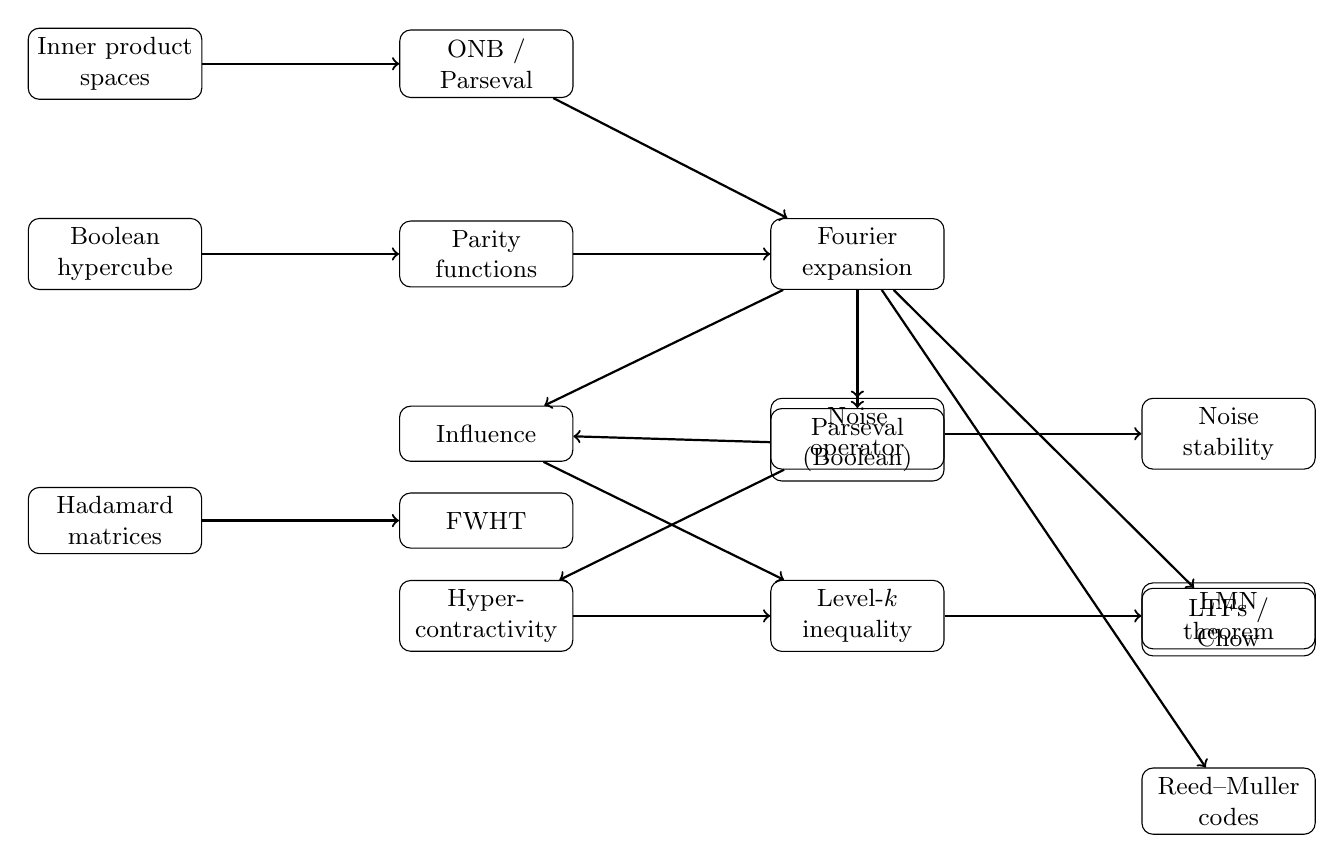
\begin{tikzpicture}[
  node distance=1.5cm and 2.5cm,
  every node/.style={rectangle, draw, rounded corners, minimum width=2.2cm,
                     minimum height=0.7cm, font=\small, align=center},
  arrow/.style={->, thick}
]
  \node (ip) {Inner product\\spaces};
  \node (onb) [right=of ip] {ONB /\\Parseval};
  \node (hyp) [below=of ip] {Boolean\\hypercube};
  \node (par) [right=of hyp] {Parity\\functions};
  \node (fe) [right=of par] {Fourier\\expansion};
  \node (pars) [below=of fe] {Parseval\\(Boolean)};
  \node (inf) [below=of par] {Influence};
  \node (noise) [right=of inf] {Noise\\operator};
  \node (stab) [right=of noise] {Noise\\stability};
  \node (hc) [below=of inf] {Hyper-\\contractivity};
  \node (lk) [right=of hc] {Level-$k$\\inequality};
  \node (lmn) [right=of lk] {LMN\\theorem};
  \node (had) [below=2.5cm of hyp] {Hadamard\\matrices};
  \node (fwht) [right=of had] {FWHT};
  \node (ltf) [below=of stab] {LTFs /\\Chow};
  \node (rm) [below=of lmn] {Reed--Muller\\codes};

  \draw[arrow] (ip) -- (onb);
  \draw[arrow] (hyp) -- (par);
  \draw[arrow] (onb) -- (fe);
  \draw[arrow] (par) -- (fe);
  \draw[arrow] (fe) -- (pars);
  \draw[arrow] (fe) -- (inf);
  \draw[arrow] (fe) -- (noise);
  \draw[arrow] (noise) -- (stab);
  \draw[arrow] (pars) -- (inf);
  \draw[arrow] (hc) -- (lk);
  \draw[arrow] (noise) -- (hc);
  \draw[arrow] (lk) -- (lmn);
  \draw[arrow] (had) -- (fwht);
  \draw[arrow] (fe) -- (ltf);
  \draw[arrow] (fe) -- (rm);
  \draw[arrow] (inf) -- (lk);
\end{tikzpicture}
\end{center}


% ──────────────────────────────────────────────────────────────────────
\section{Suggestions for Further Reading}\label{sec:further-reading}

\begin{enumerate}
  \item \textbf{Boolean Fourier analysis (comprehensive):}
    \citet{odonnell2014analysis}. Available free at arXiv:2105.10386.
    Chapters~1--5 cover the core material; Chapters~8--10 cover
    hypercontractivity and the LMN theorem.

  \item \textbf{Boolean Fourier analysis (short introduction):}
    \citet{dewolf2008brief}. A 20-page survey covering the essentials.
    Freely available at the Theory of Computing library.

  \item \textbf{Noise sensitivity and social choice:}
    \citet{benjamini1999noise}. The foundational paper connecting noise
    sensitivity to percolation theory. Beautiful mathematics.

  \item \textbf{Hadamard matrices:}
    \citet{horadam2007hadamard}. Comprehensive treatment of Hadamard
    matrices and their applications.

  \item \textbf{Walsh functions and signal processing:}
    \citet{beauchamp1984walsh}. The classical reference for Walsh
    functions in engineering.

  \item \textbf{Reed--Muller codes:}
    \citet{macwilliams1977theory}, Chapters~13--14. The standard
    reference for algebraic coding theory.

  \item \textbf{Fourier analysis on finite groups:}
    \citet{terras1999fourier}. Develops Fourier analysis on general
    finite groups with many applications.

  \item \textbf{Probability (CLT, Berry--Ess\'een):}
    \citet{durrett2019probability}, Chapter~3. Or
    \citet{feller1971introduction}, Volume~2, Chapter~XVI.

  \item \textbf{Binary neural networks:}
    Start with \citet{courbariaux2015binaryconnect}, then
    \citet{rastegari2016xnor} and \citet{hubara2016binarized} for the
    foundational work. \citet{wang2023bitnet} and \citet{ma2024era} for
    the state of the art.
\end{enumerate}


\bibliographystyle{plainnat}
\bibliography{guide_references}

\end{document}
